\chapter{Результаты проведённых расчётов} \label{ch3}


В данном разделе представлены результаты расчётов. Получены первые 10 собственных частот и форм рассматриваемого изделия (рис. \ref{fig:mod1}-\ref{fig:mod10}).

Для того, чтобы получить наглядную количественную картину направлений, в которых будет возбуждаться каждая из собственных форм, получены значения параметров вклада и эффективных масс рассматриваемого изделия. Результаты представлены на рис. \ref{fig:part-factor}-\ref{fig:cum-effective-mass}.

\begin{figure}[H] 
	\center
	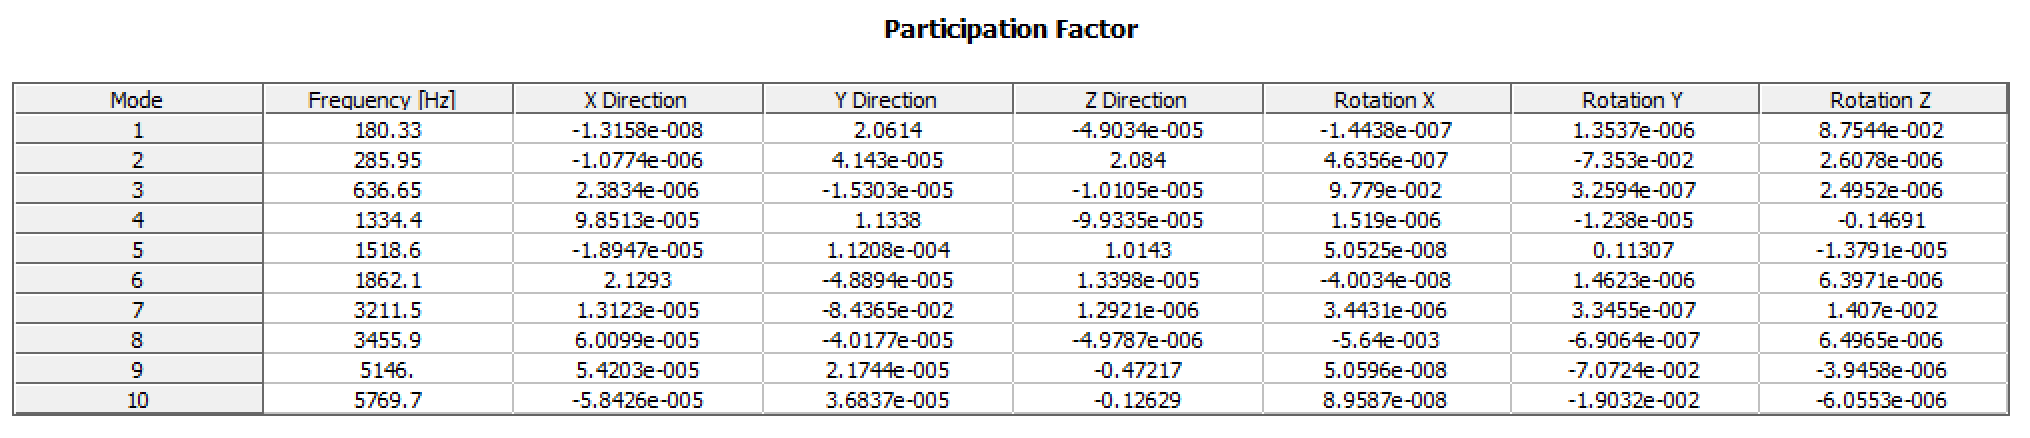
\includegraphics[width=\textwidth]{images/part-factor.png}
	\caption{Значения параметров вклада в каждую из собственных форм}
	\label{fig:part-factor}
\end{figure}

\begin{figure}[H] 
	\center
	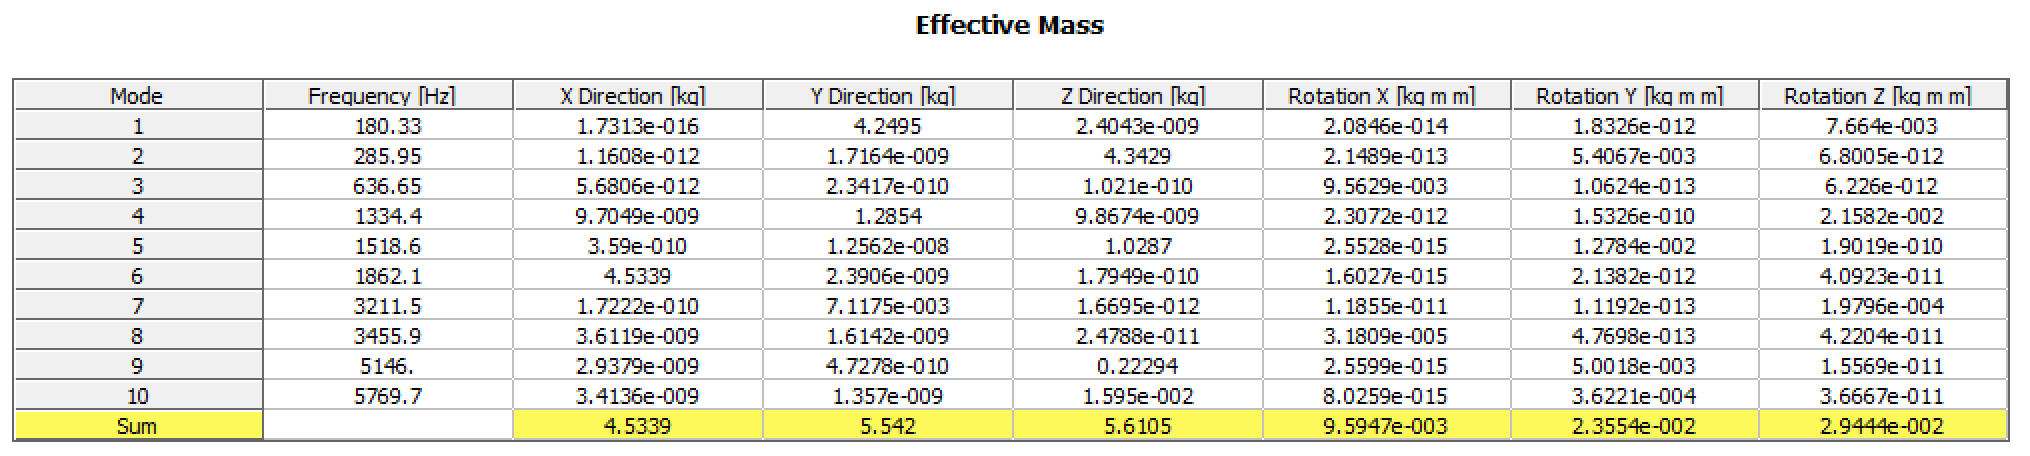
\includegraphics[width=\textwidth]{images/effective-mass.png}
	\caption{Значения эффективных масс для каждой из собственных форм}
	\label{fig:effective-mass}
\end{figure}

\begin{figure}[H] 
	\center
	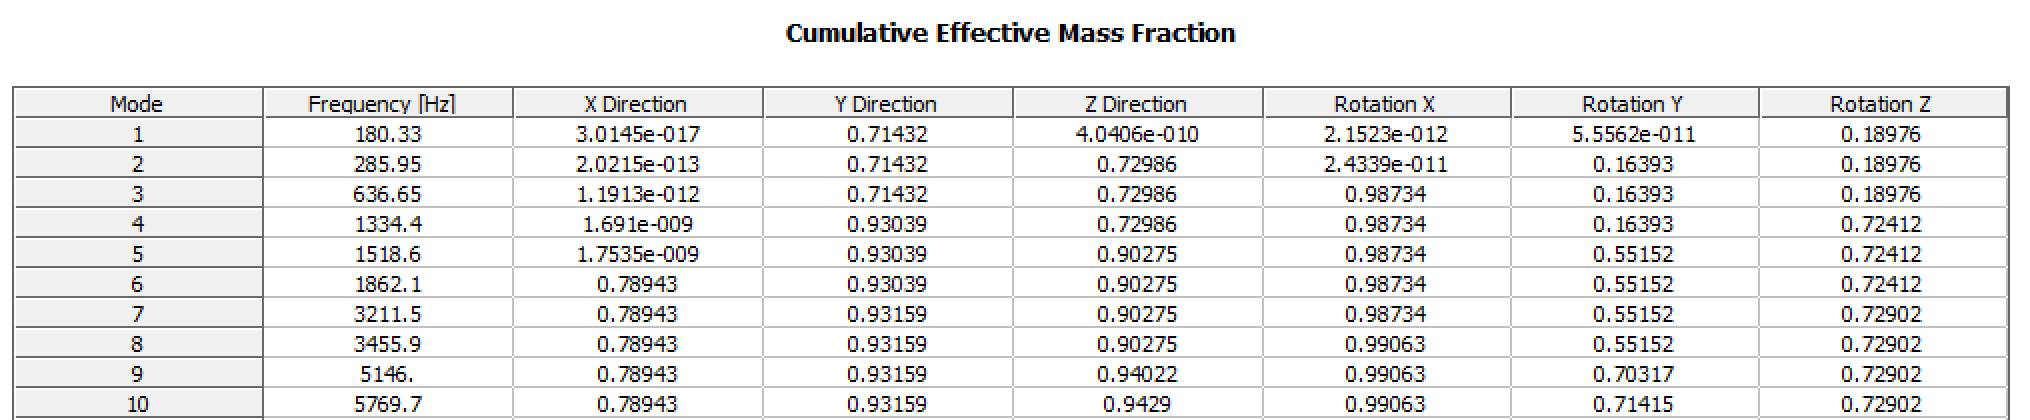
\includegraphics[width=\textwidth]{images/cum-effective-mass.png}
	\caption{Значения кумулятивных эффективных масс на каждой из собственных форм}
	\label{fig:cum-effective-mass}
\end{figure}


\begin{figure}[H] 
	\center
	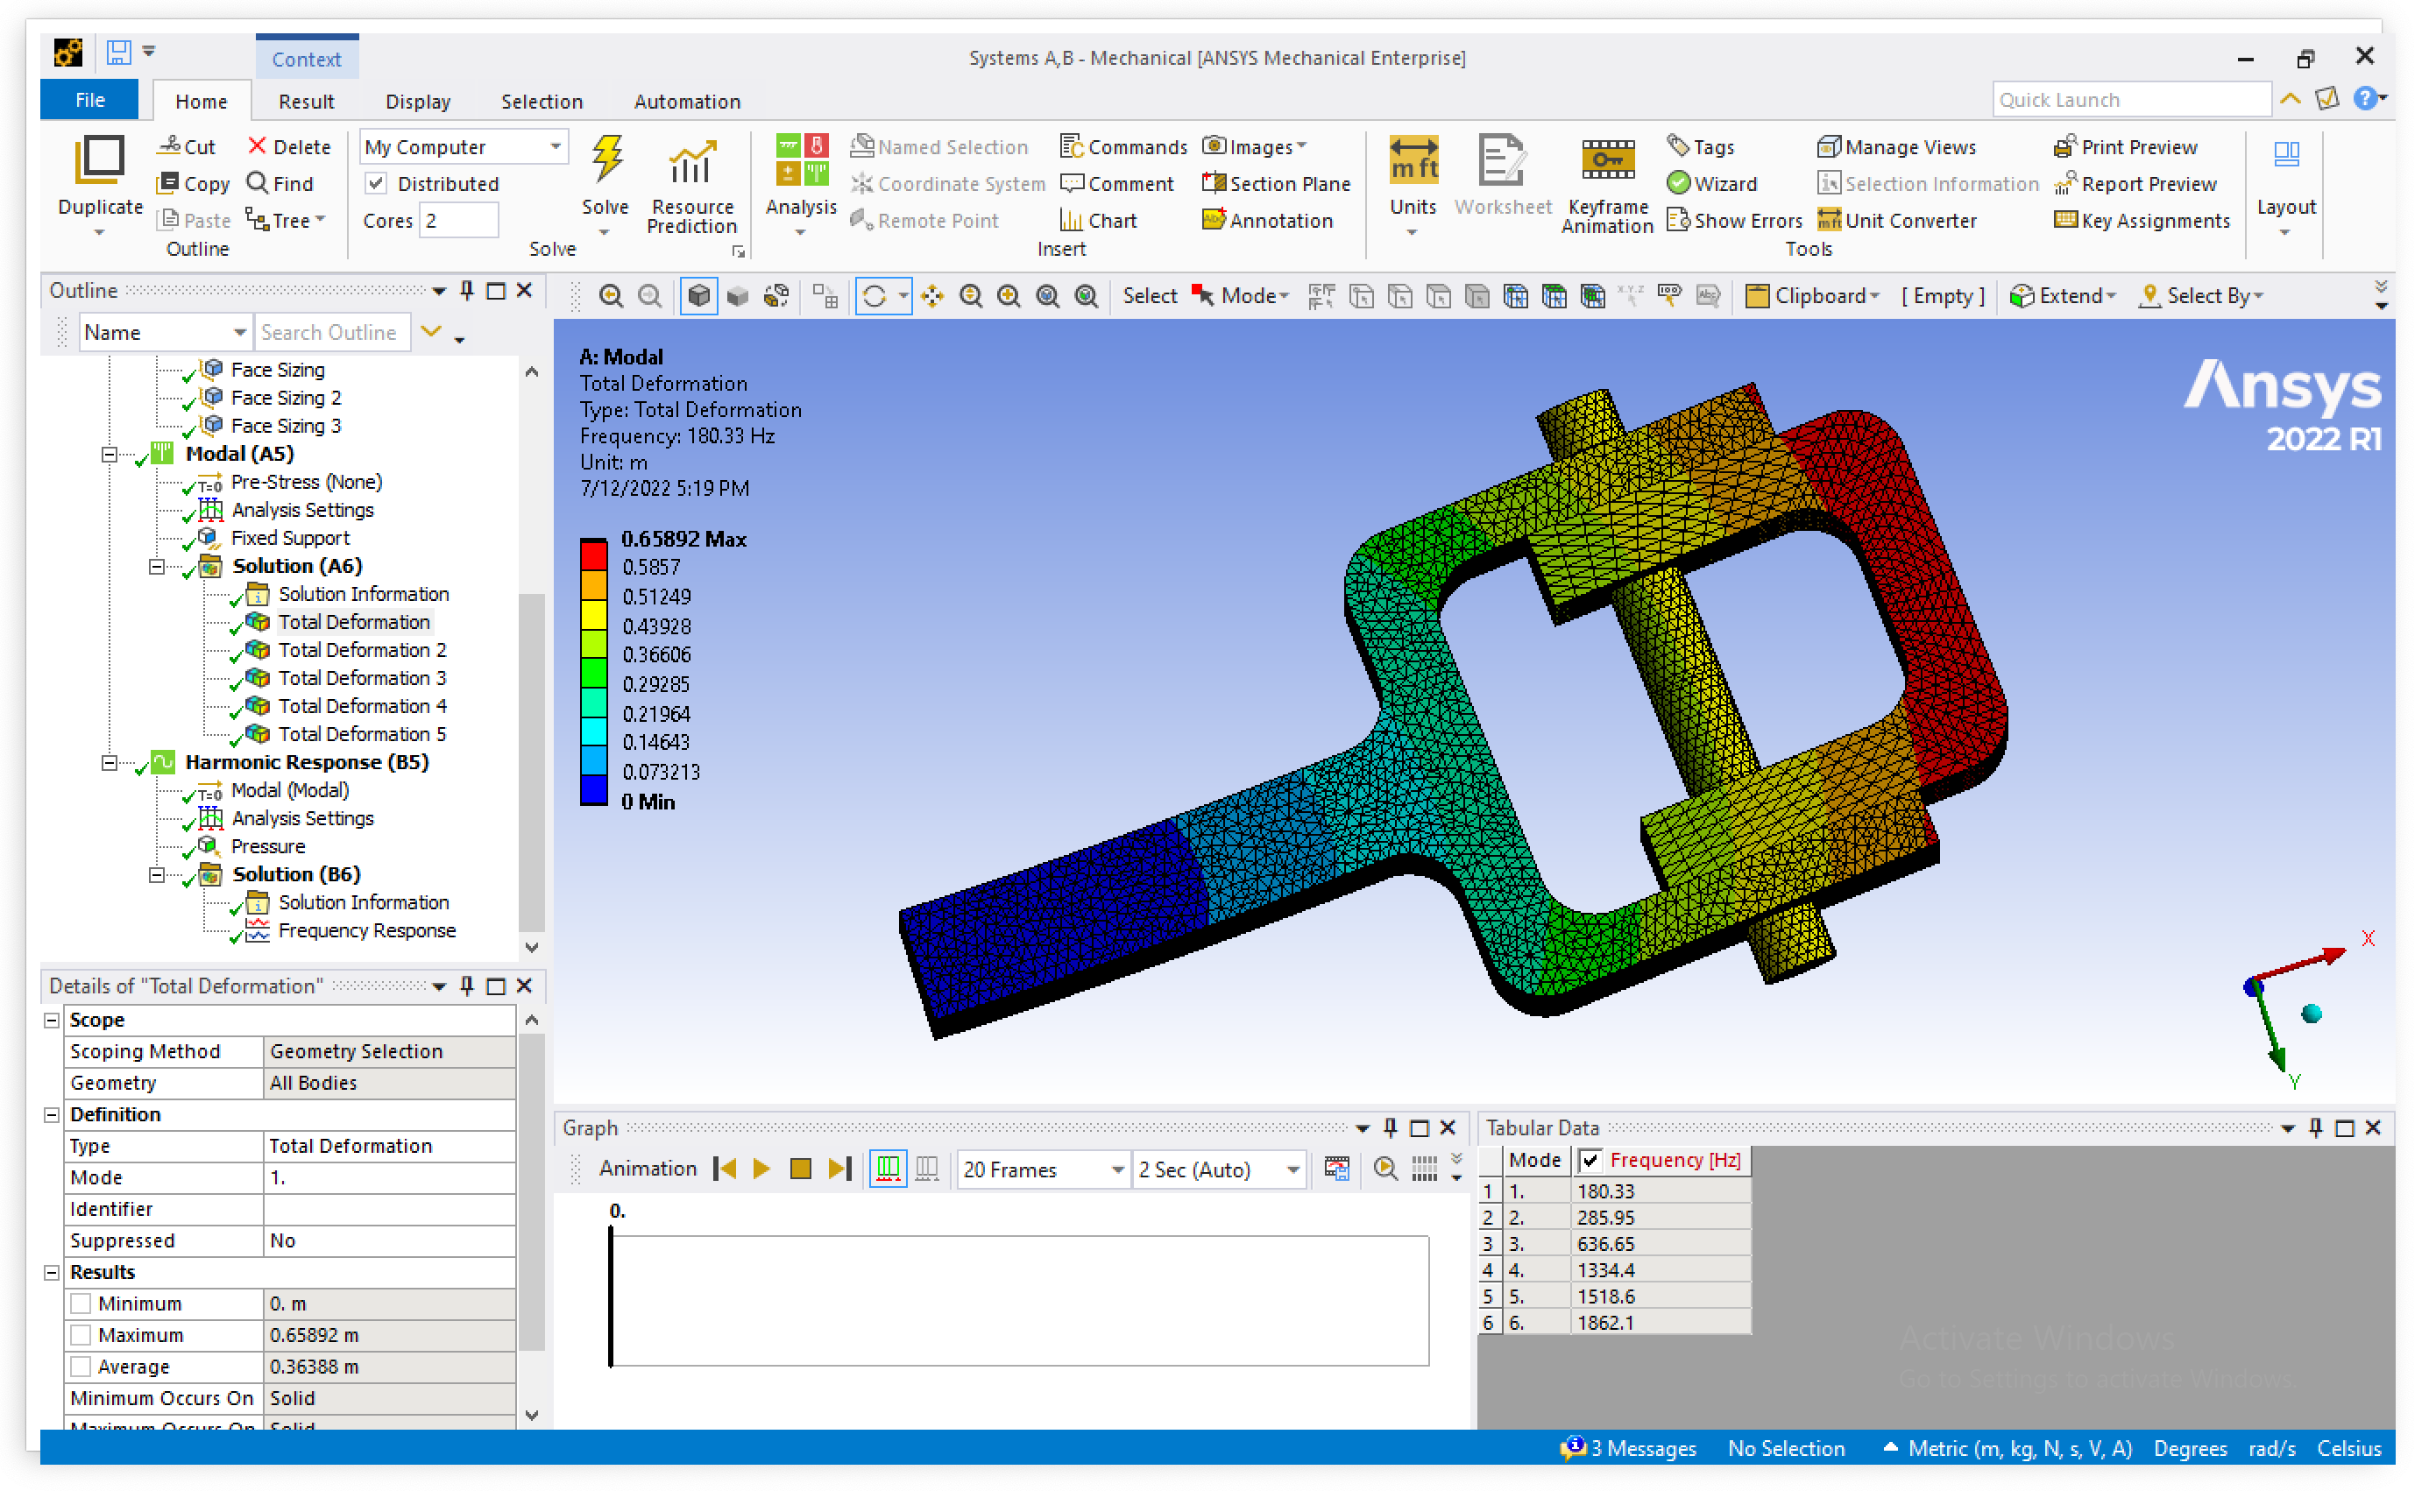
\includegraphics[width=\textwidth]{images/mod1.png}
	\caption{Деформации при первой собственной частоте (преимущественно перемещения вдоль оси Oy и вращение вокруг оси Oz)}
	\label{fig:mod1}
\end{figure}

\begin{figure}[H] 
	\center
	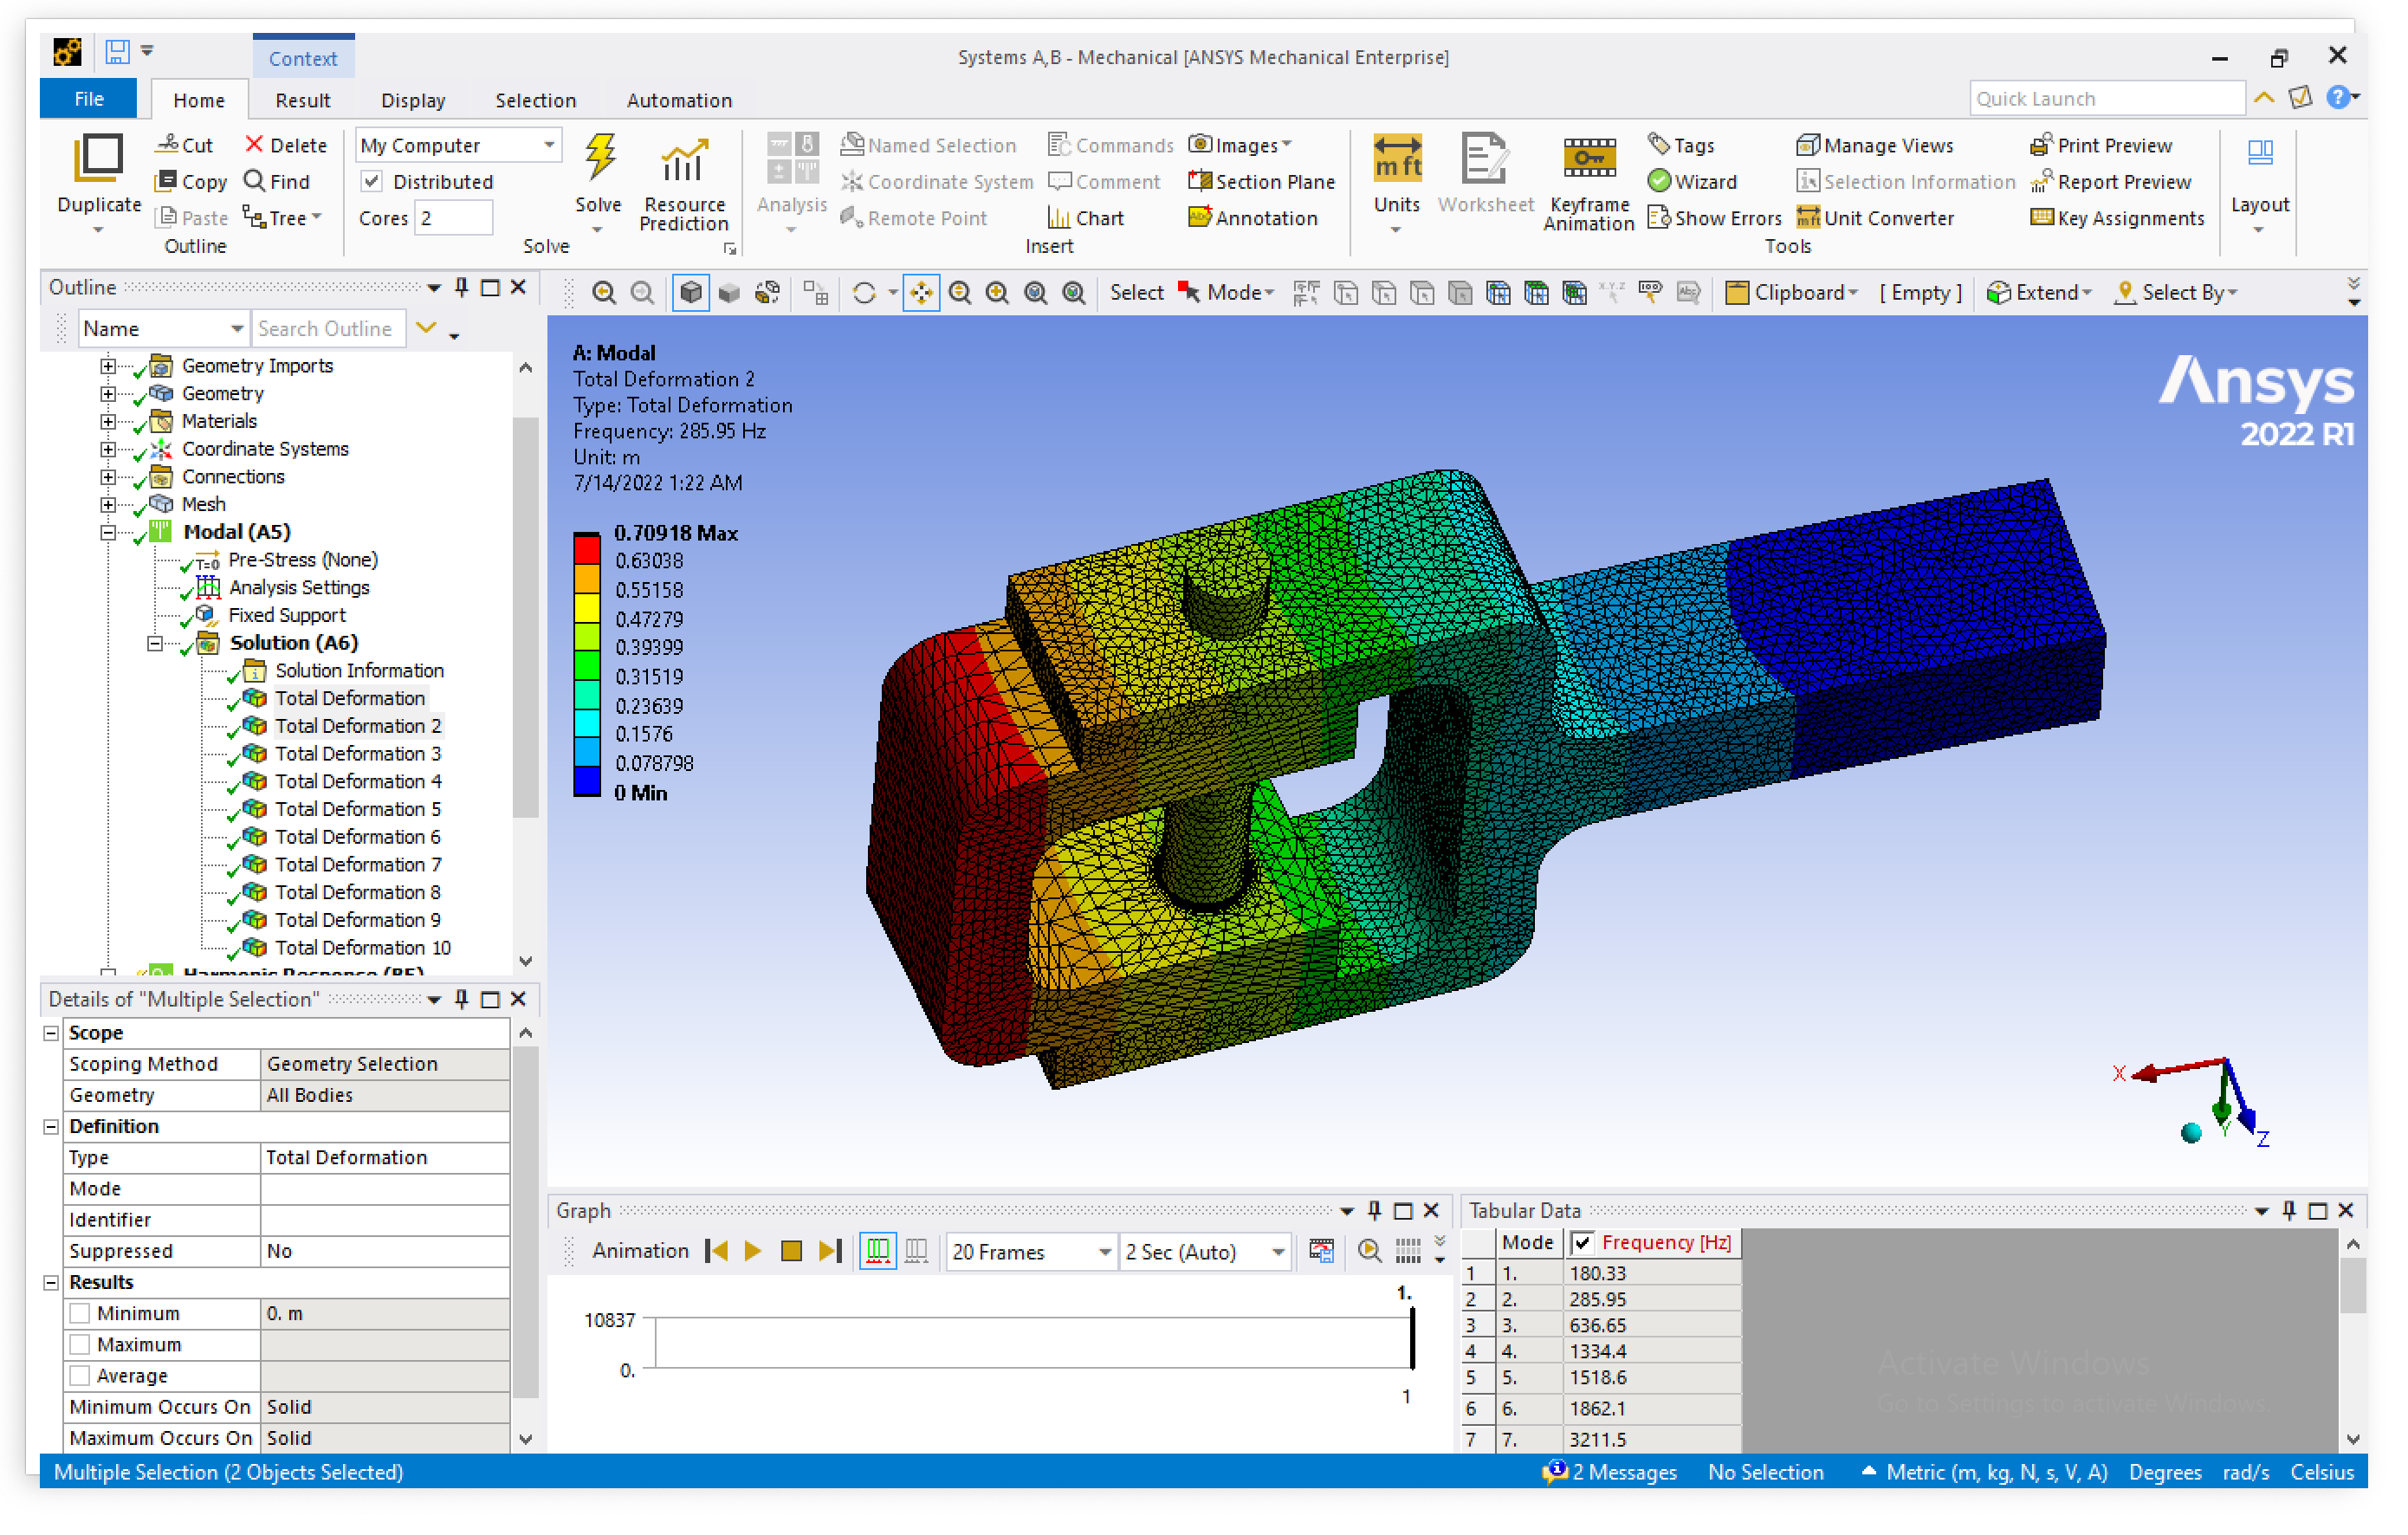
\includegraphics[width=\textwidth]{images/mod2.png}
	\caption{Деформации при второй собственной частоте (преимущественно перемещение вдоль оси Oz и вращение вокруг оси Oy)}
	\label{fig:mod2}
\end{figure}

\begin{figure}[H] 
	\center
	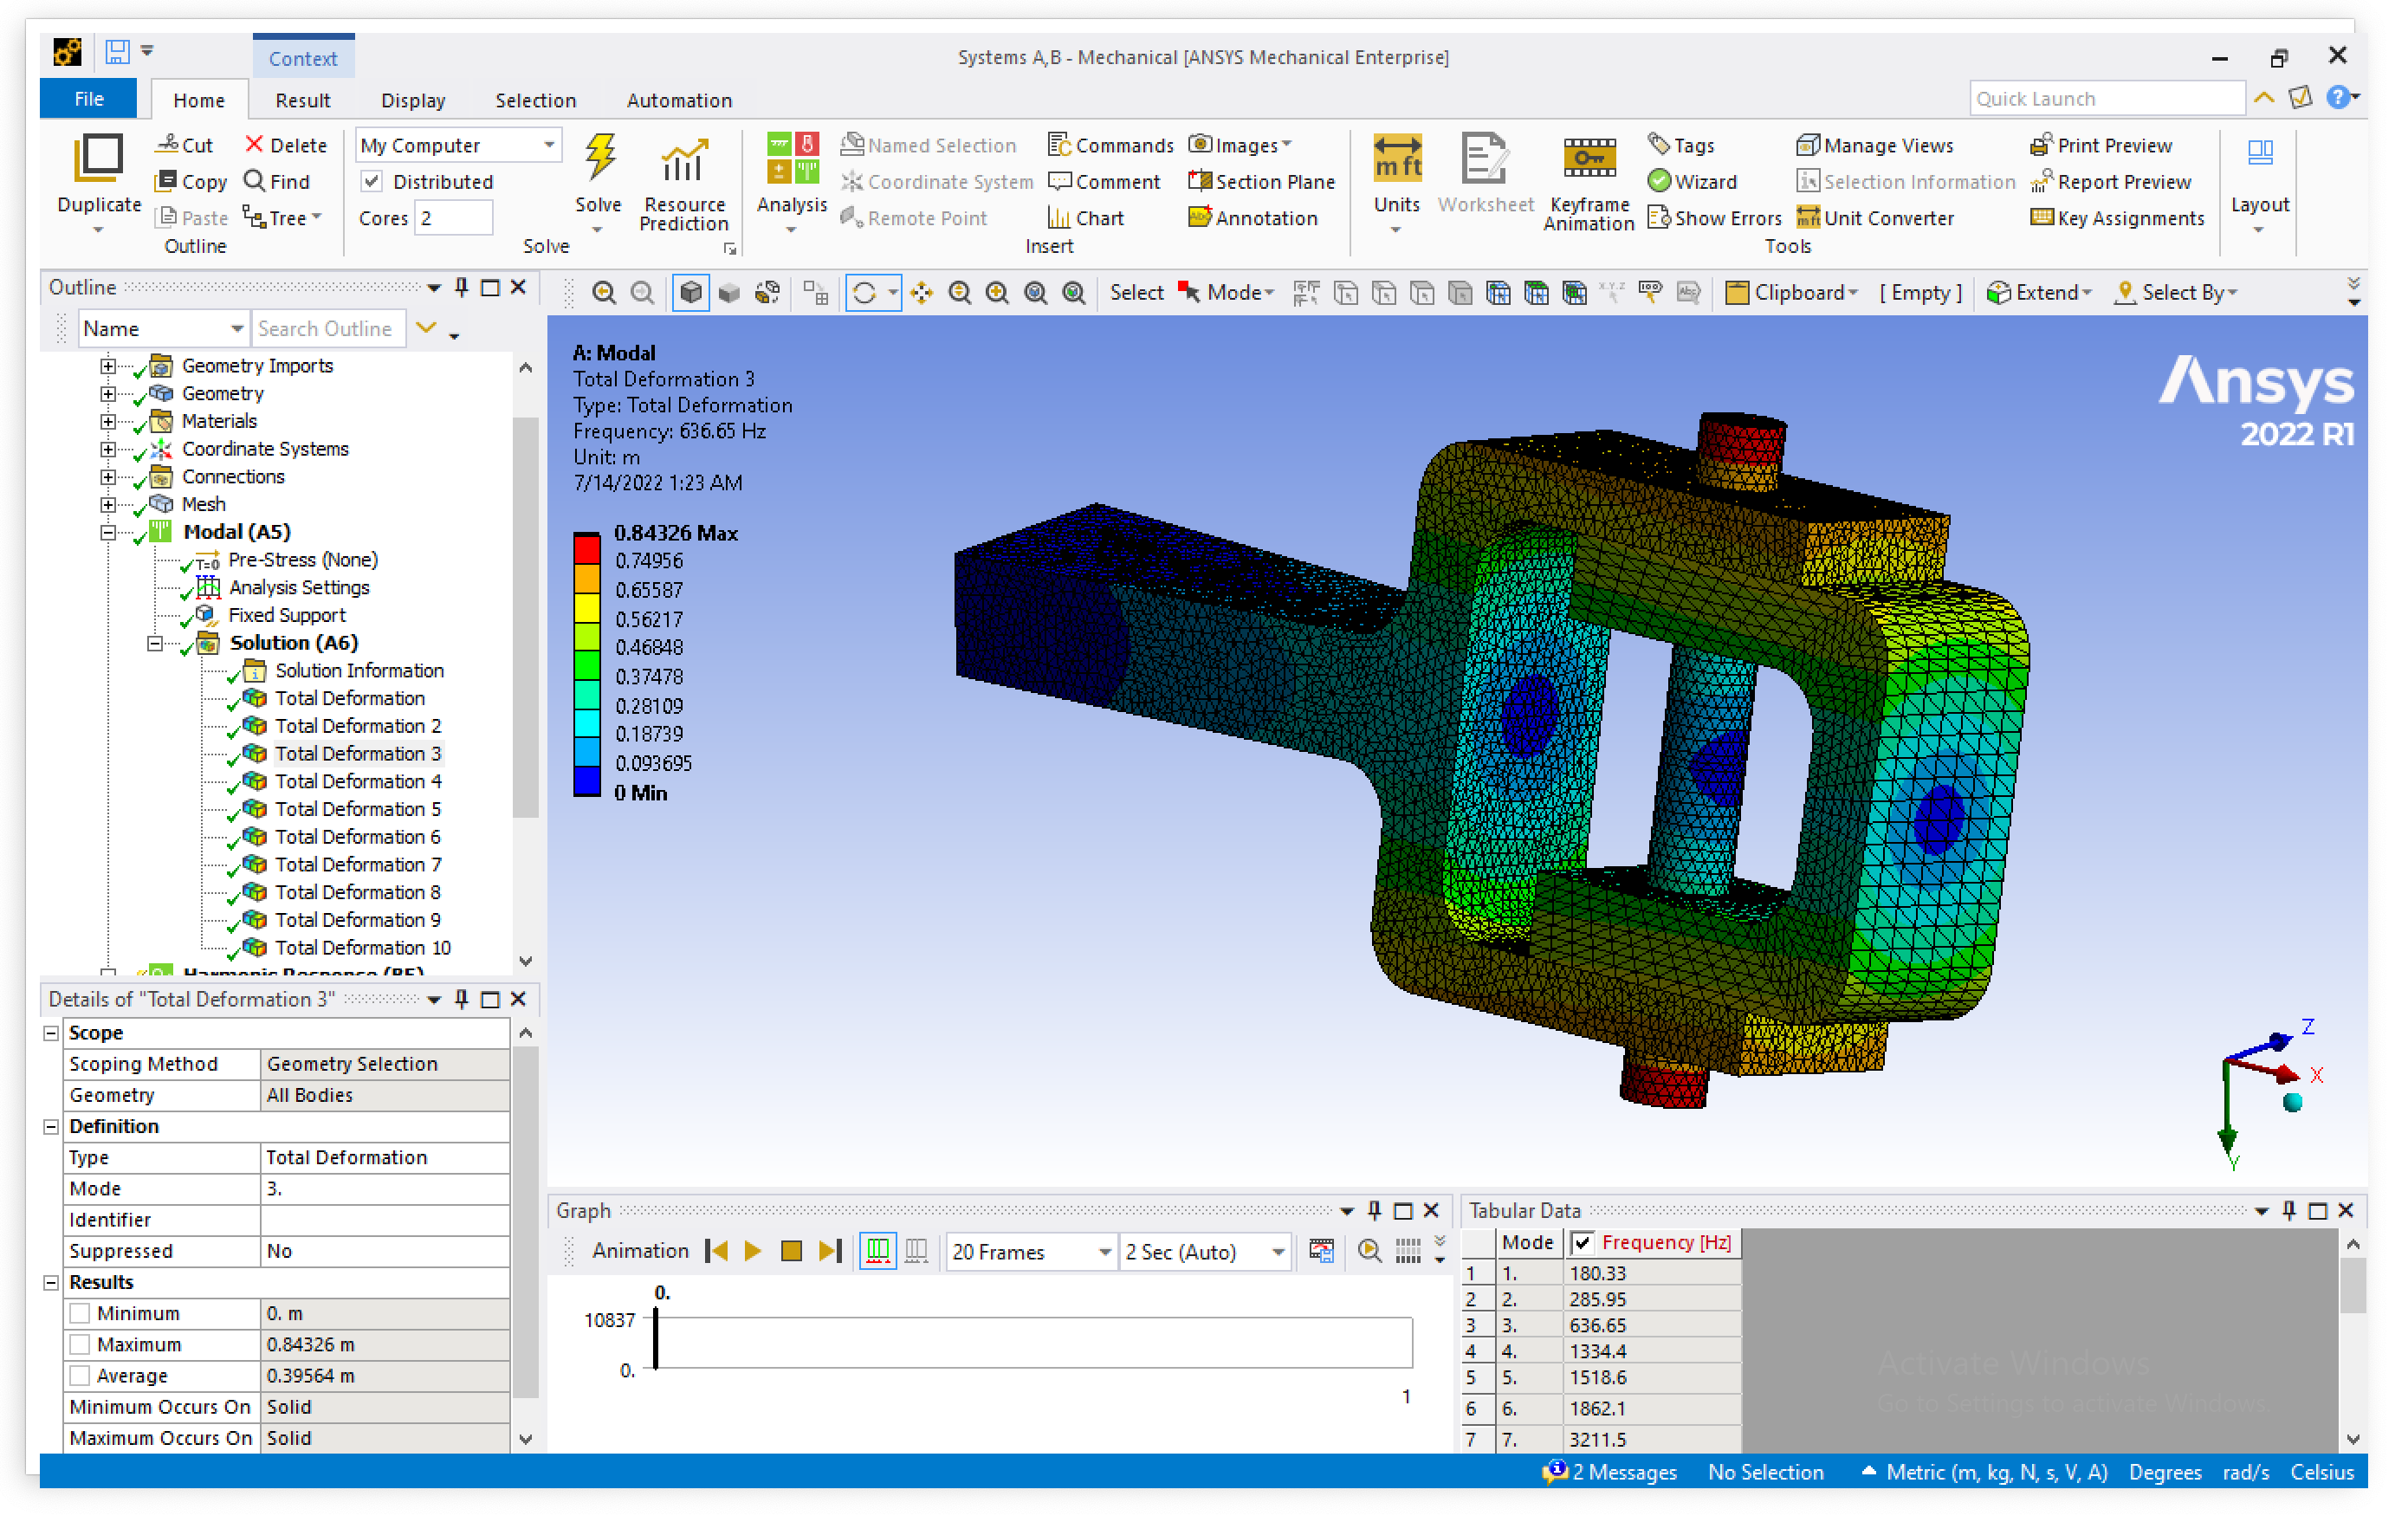
\includegraphics[width=\textwidth]{images/mod3.png}
	\caption{Деформации при третьей собственной частоте (преимущественно вращение вокруг оси Ox)}
	\label{fig:mod3}
\end{figure}

\begin{figure}[H] 
	\center
	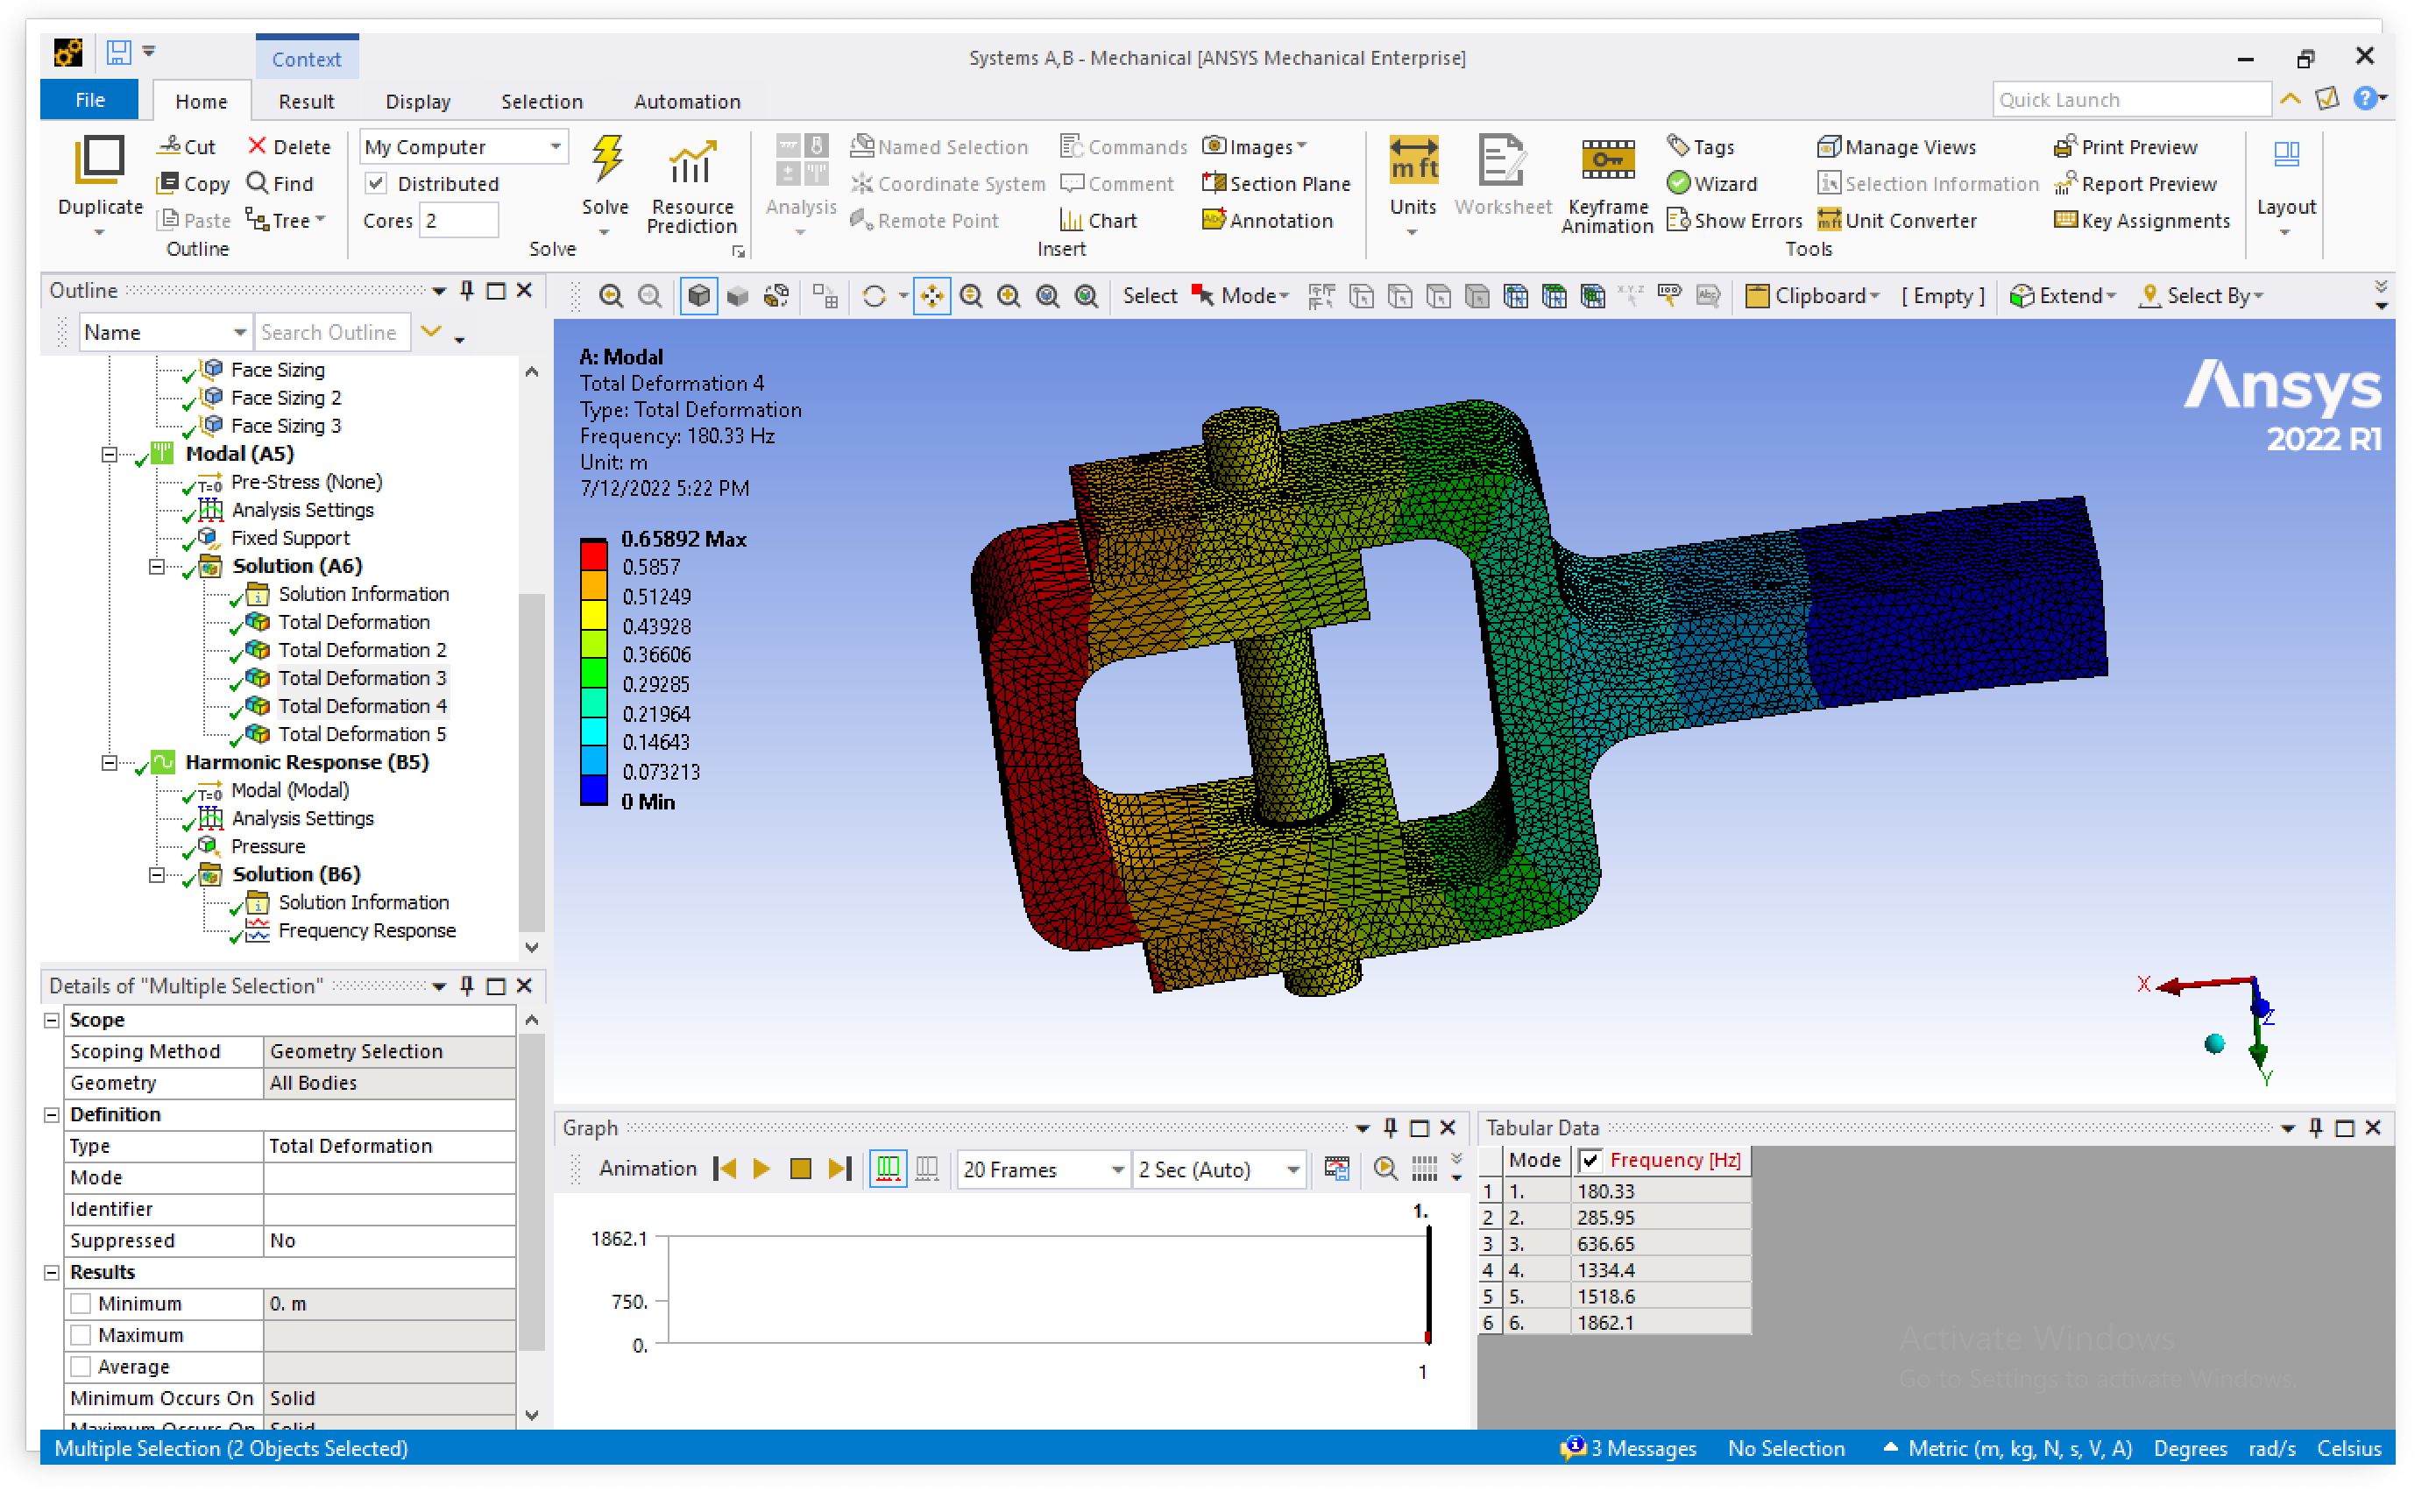
\includegraphics[width=\textwidth]{images/mod4.png}
	\caption{Деформации при четвёртой собственной частоте (преимущественно перемещение вдоль оси Oy и вращение вокруг оси Oz)}
	\label{fig:mod4}
\end{figure}

\begin{figure}[H] 
	\center
	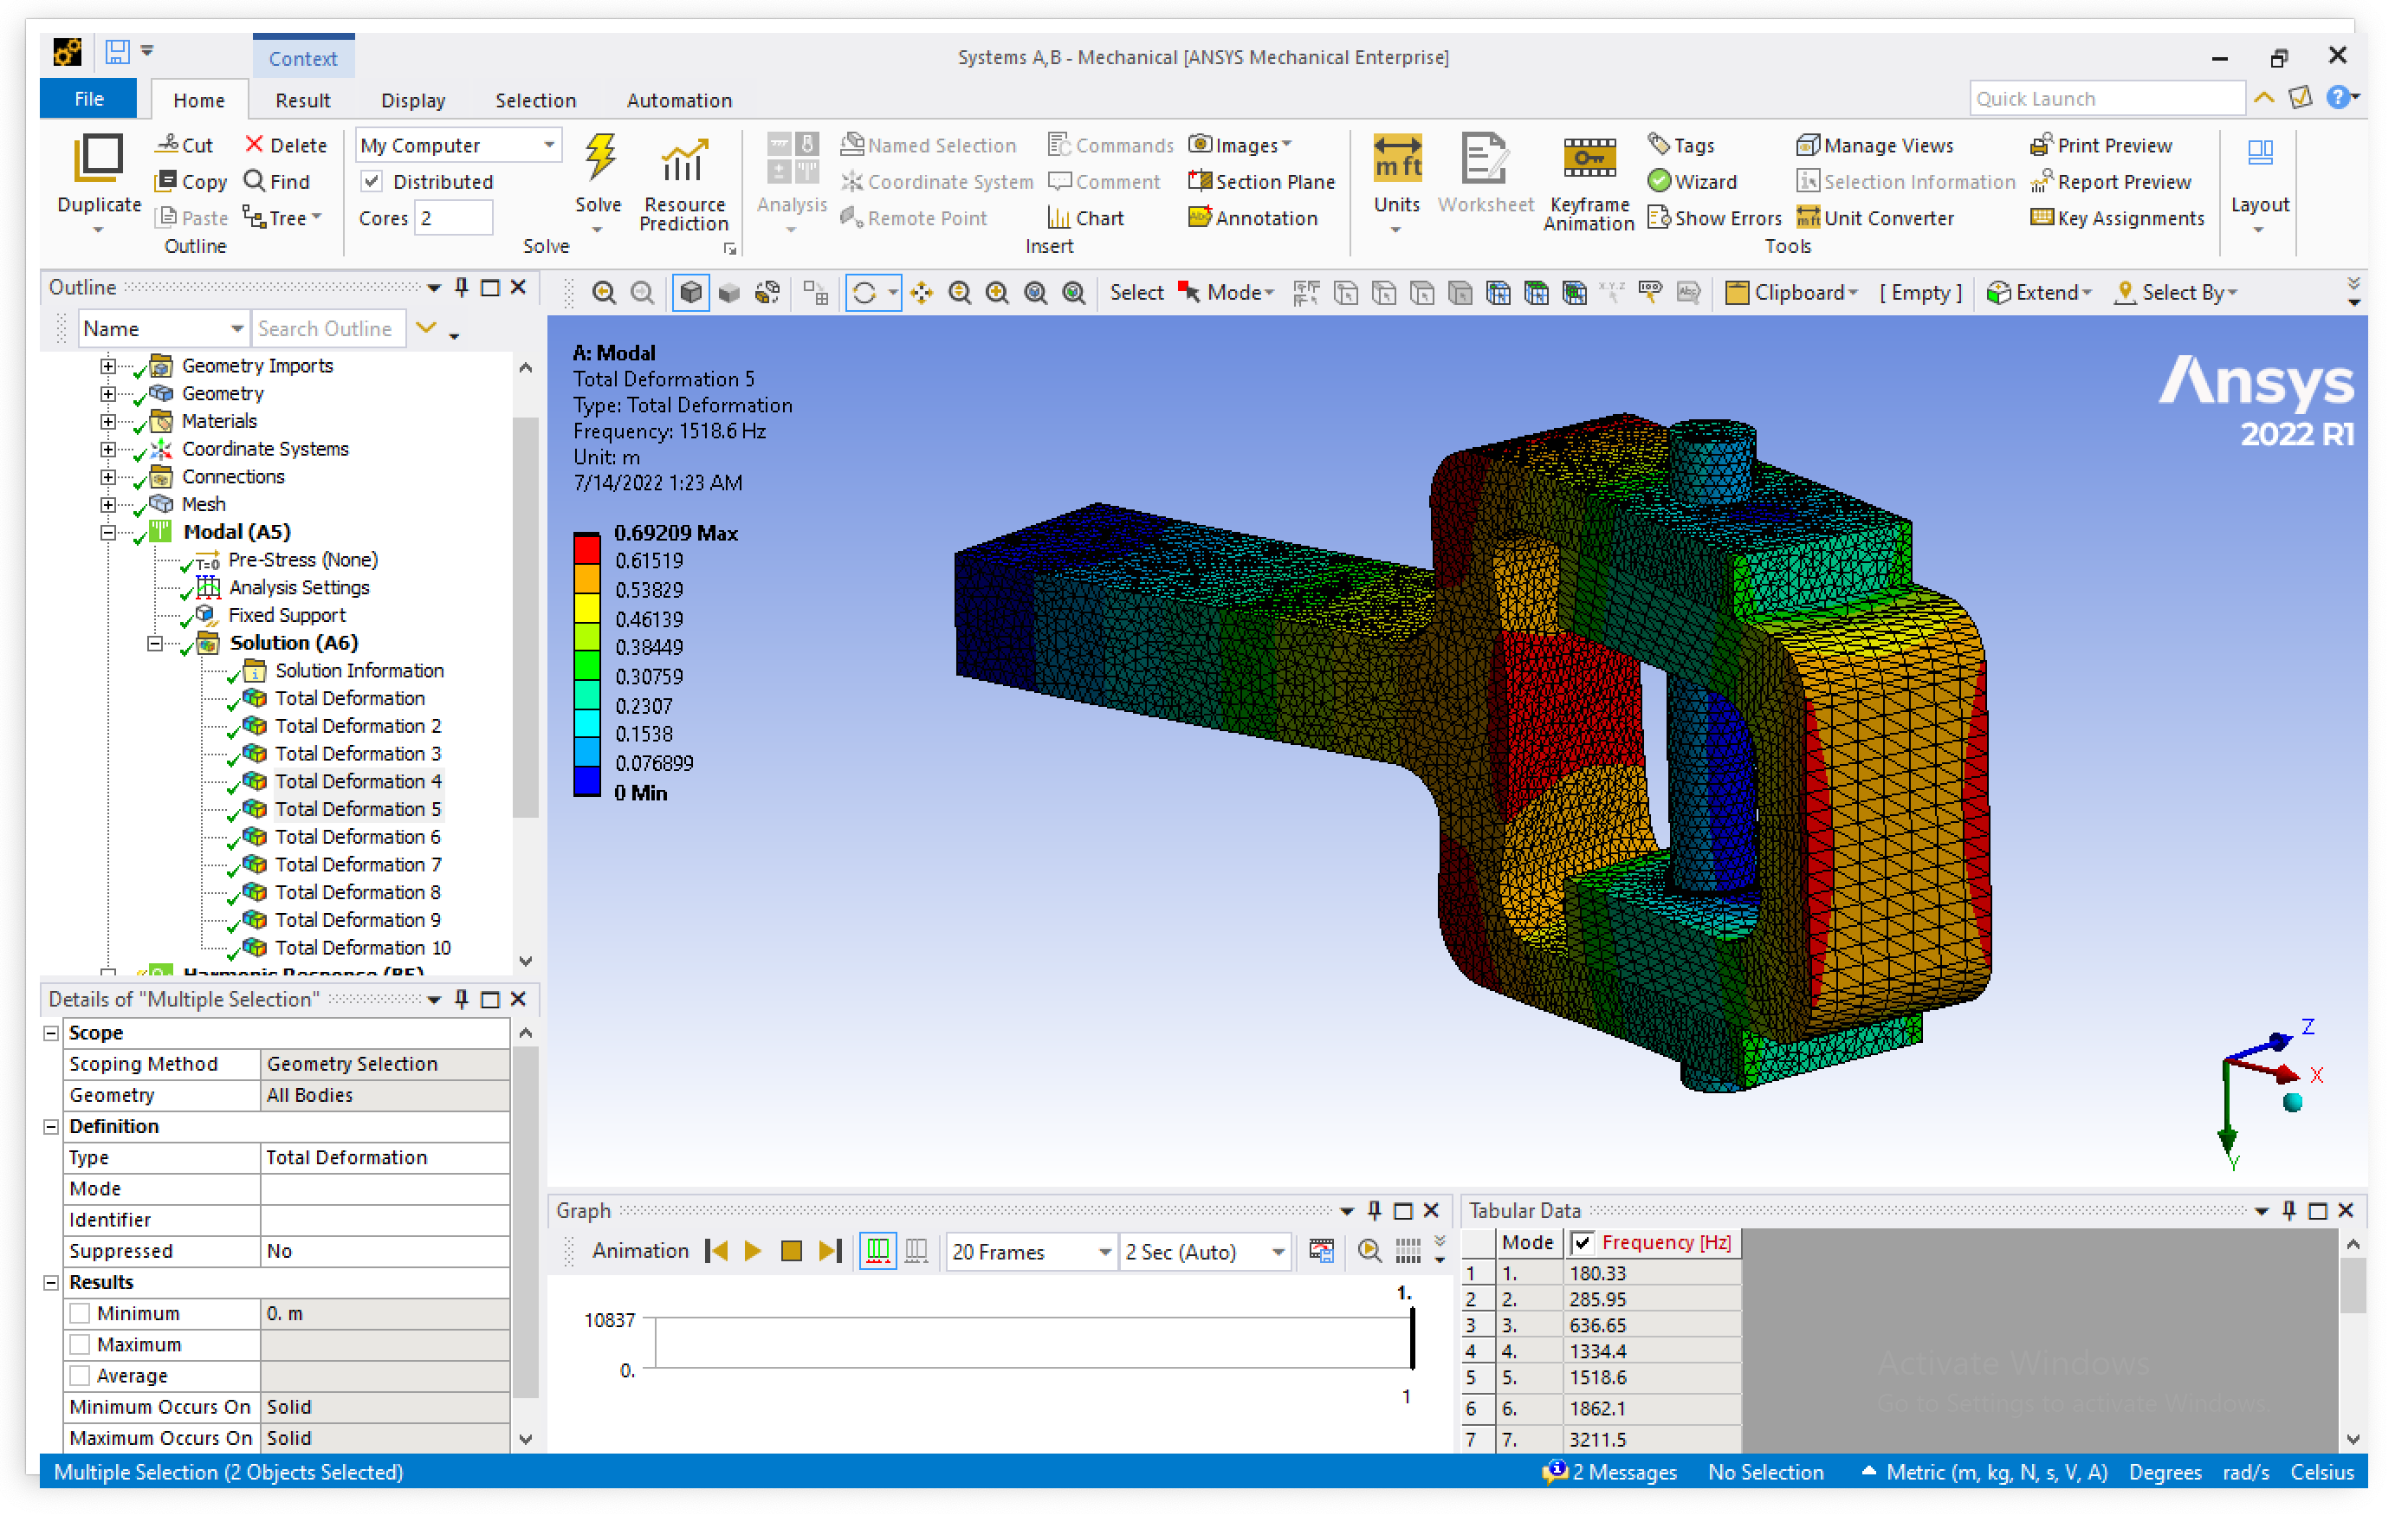
\includegraphics[width=\textwidth]{images/mod5.png}
	\caption{Деформации при пятой собственной частоте (преимущественно перемещение вдоль оси Oz и вращение вокруг оси Oy)}
	\label{fig:mod5}
\end{figure}

\begin{figure}[H] 
	\center
	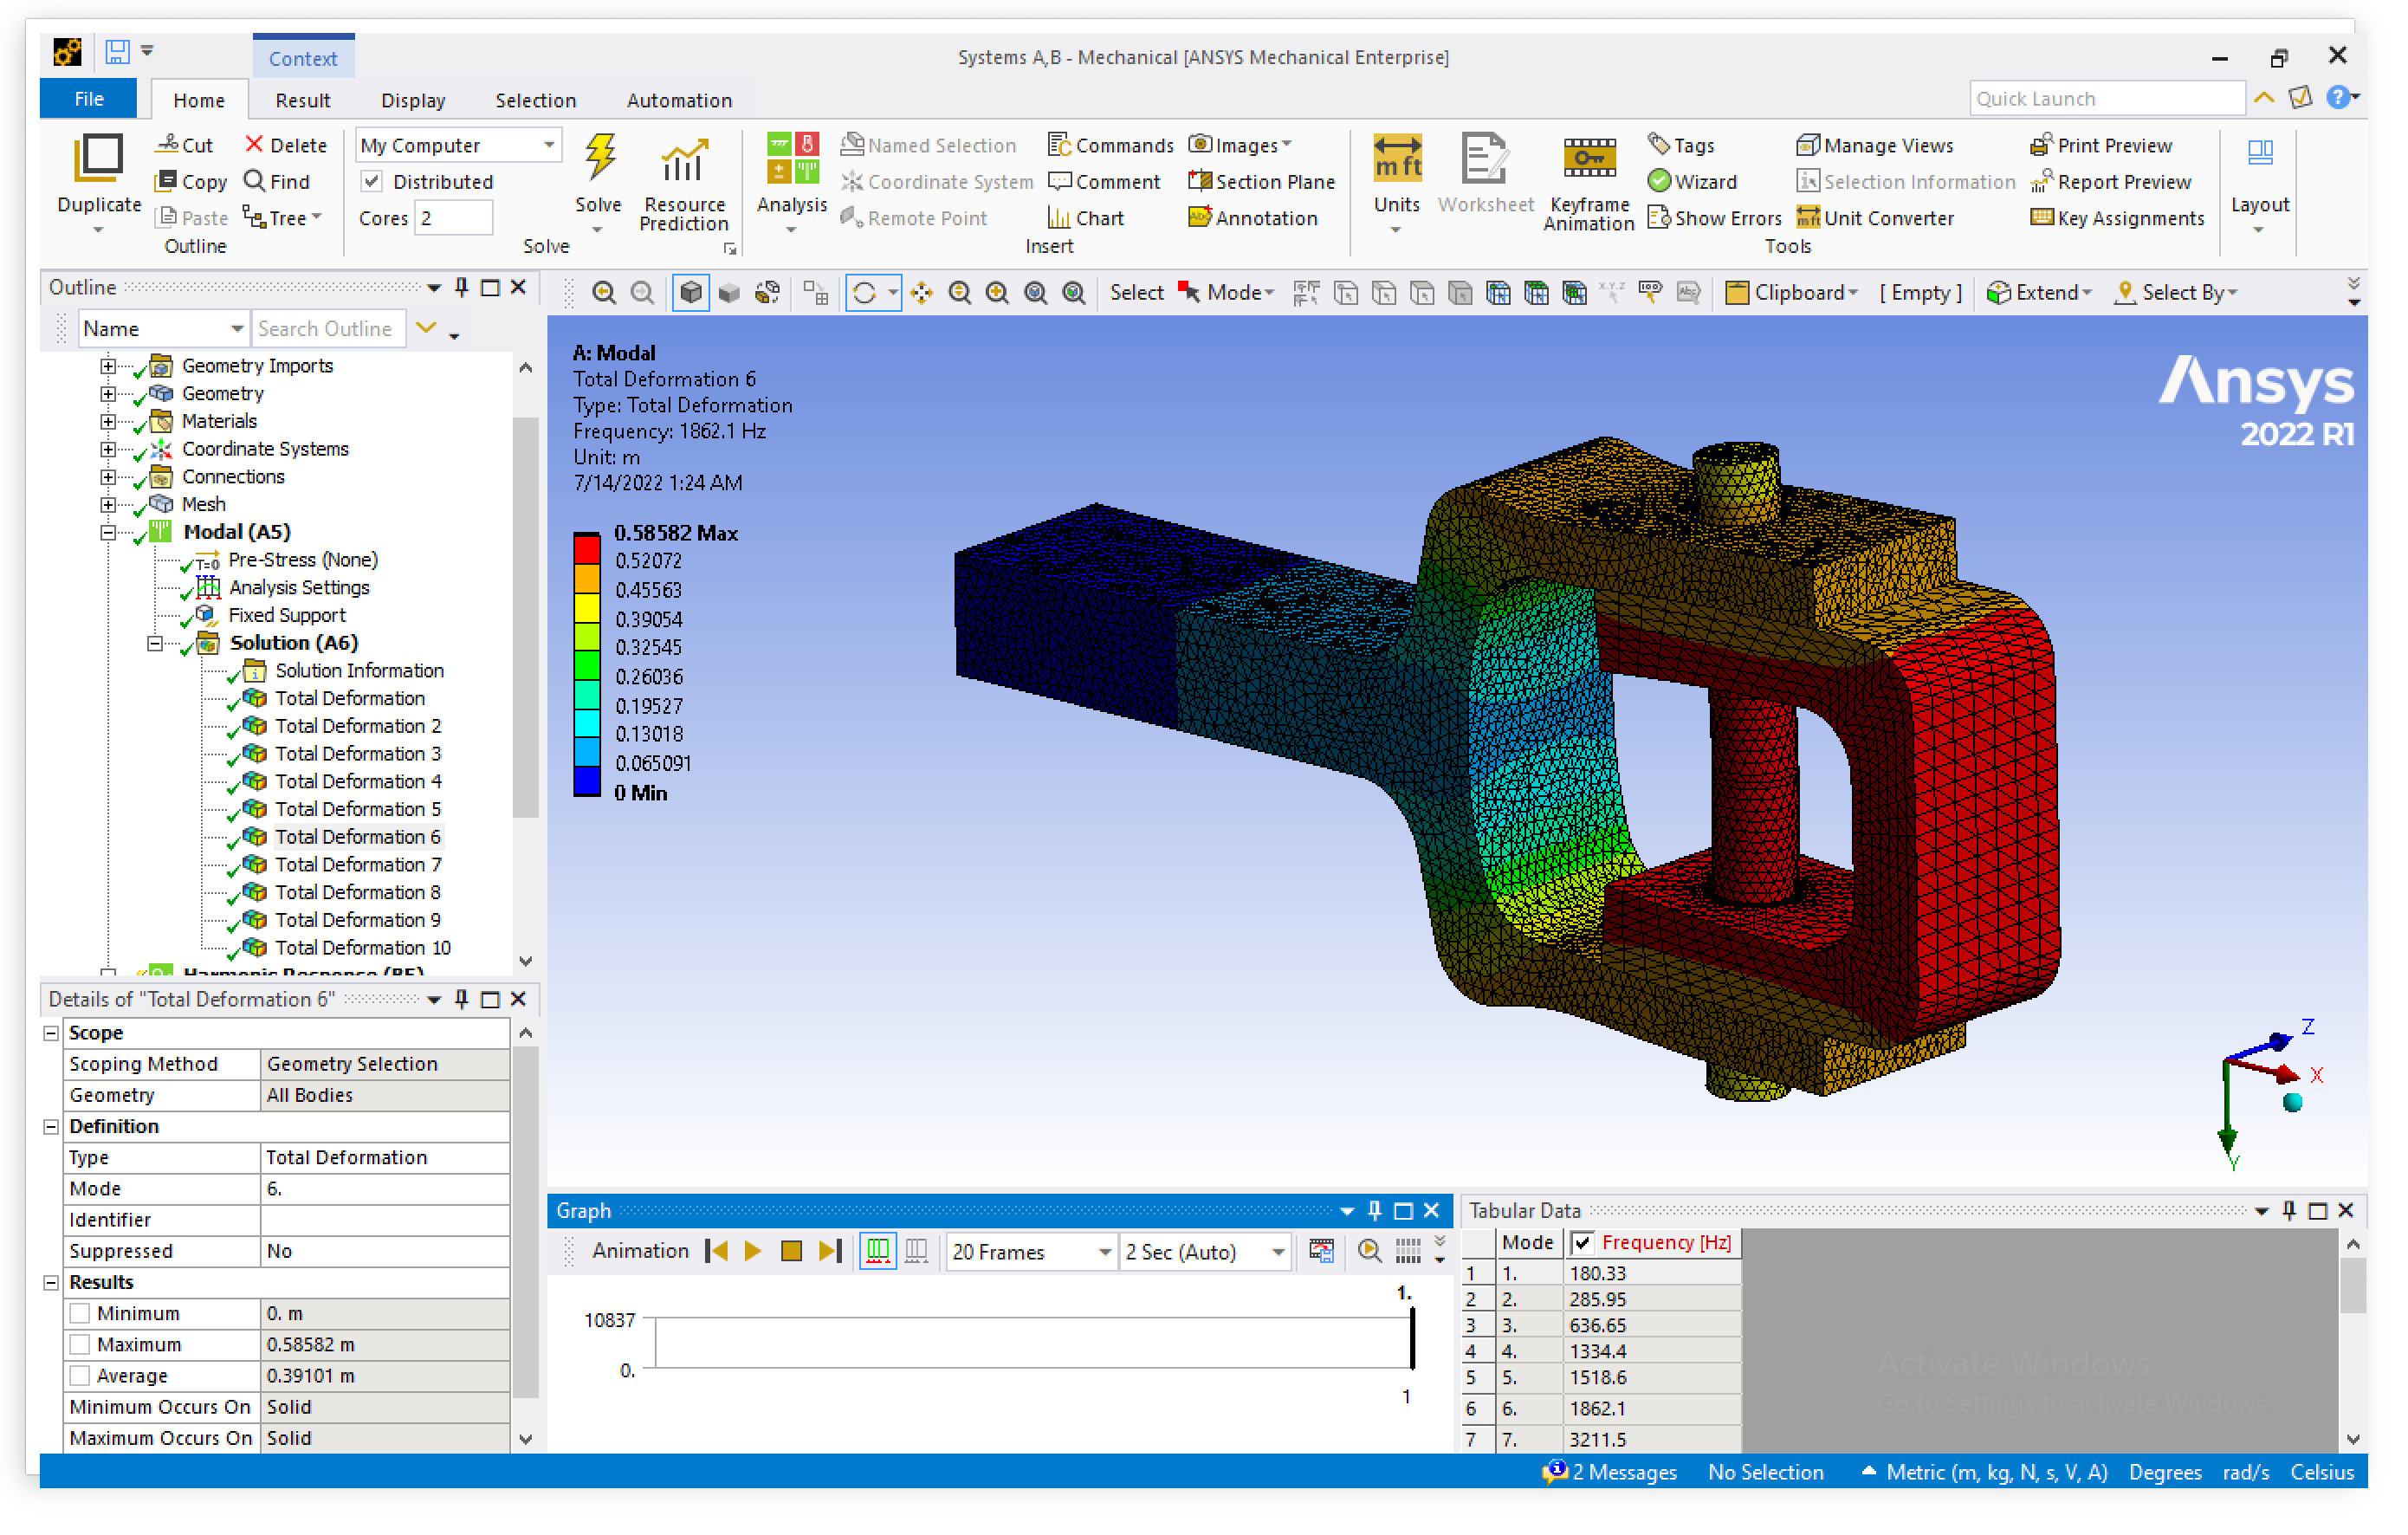
\includegraphics[width=\textwidth]{images/mod6.png}
	\caption{Деформации при шестой собственной частоте (преимущественно перемещение вдоль оси Ox)}
	\label{fig:mod6}
\end{figure}

\begin{figure}[H] 
	\center
	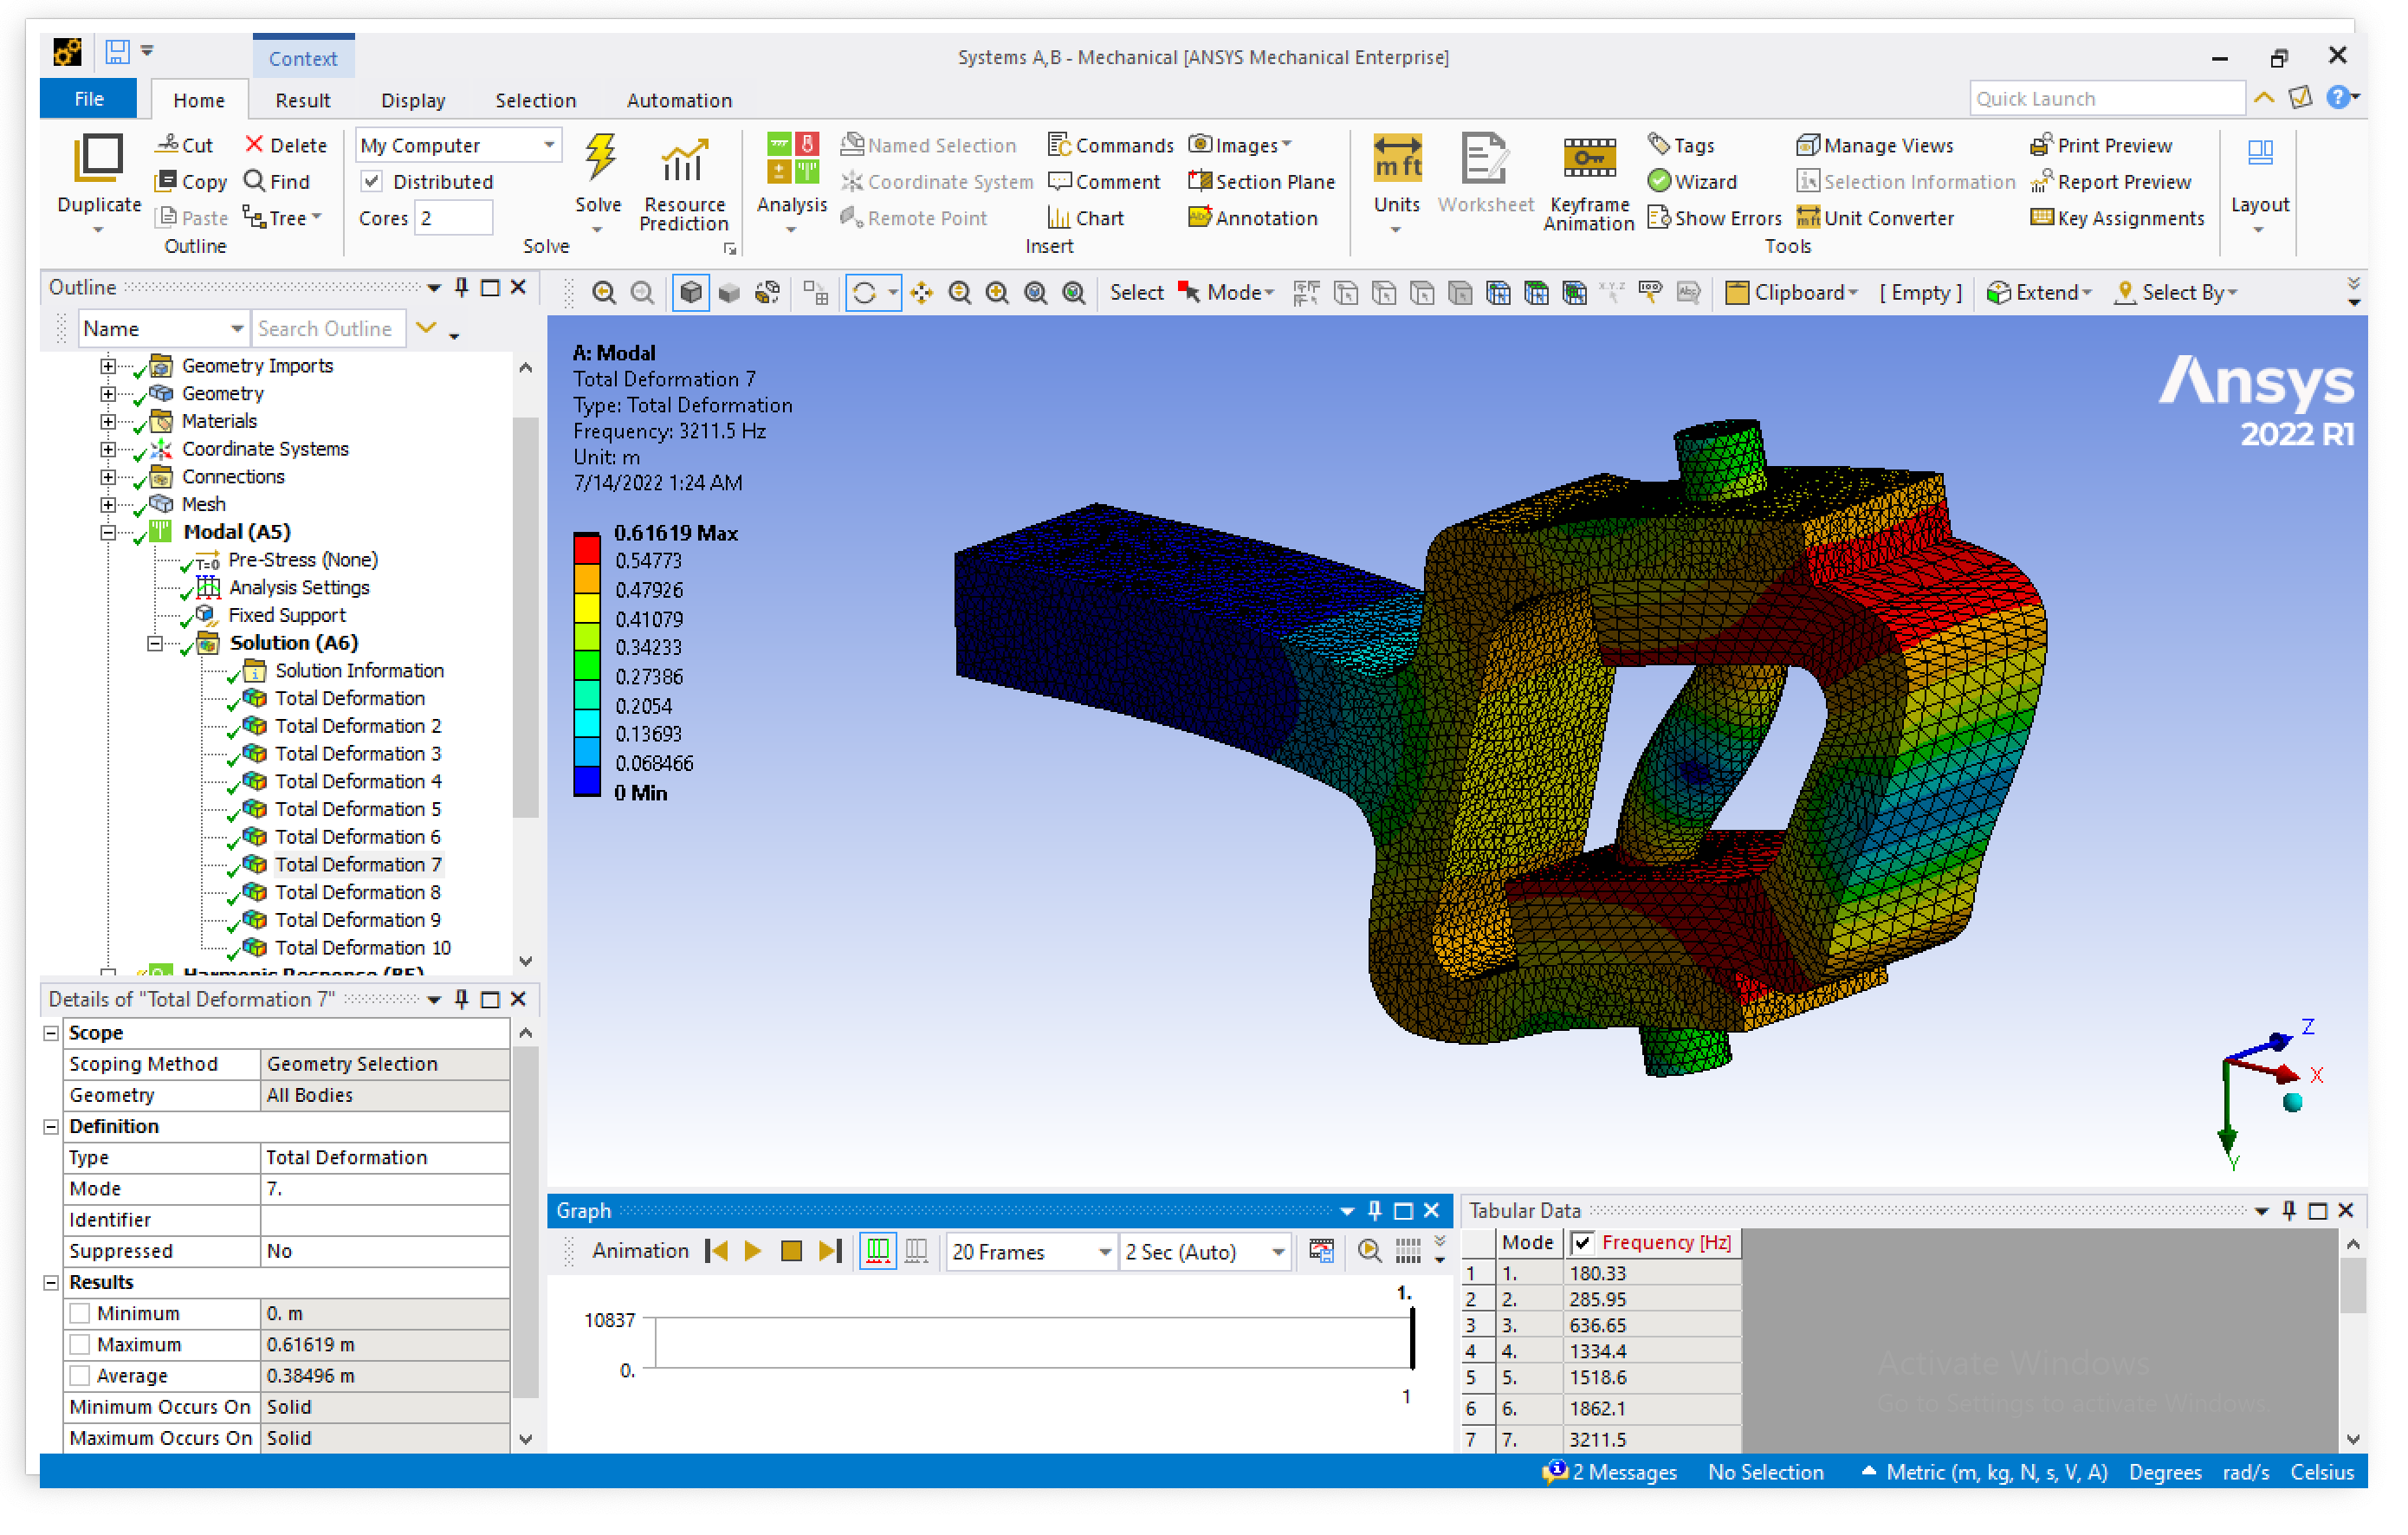
\includegraphics[width=\textwidth]{images/mod7.png}
	\caption{Деформации при седьмой собственной частоте (преимущественно перемещение вдоль оси Oy и вращение вокруг оси Oz)}
	\label{fig:mod7}
\end{figure}

\begin{figure}[H] 
	\center
	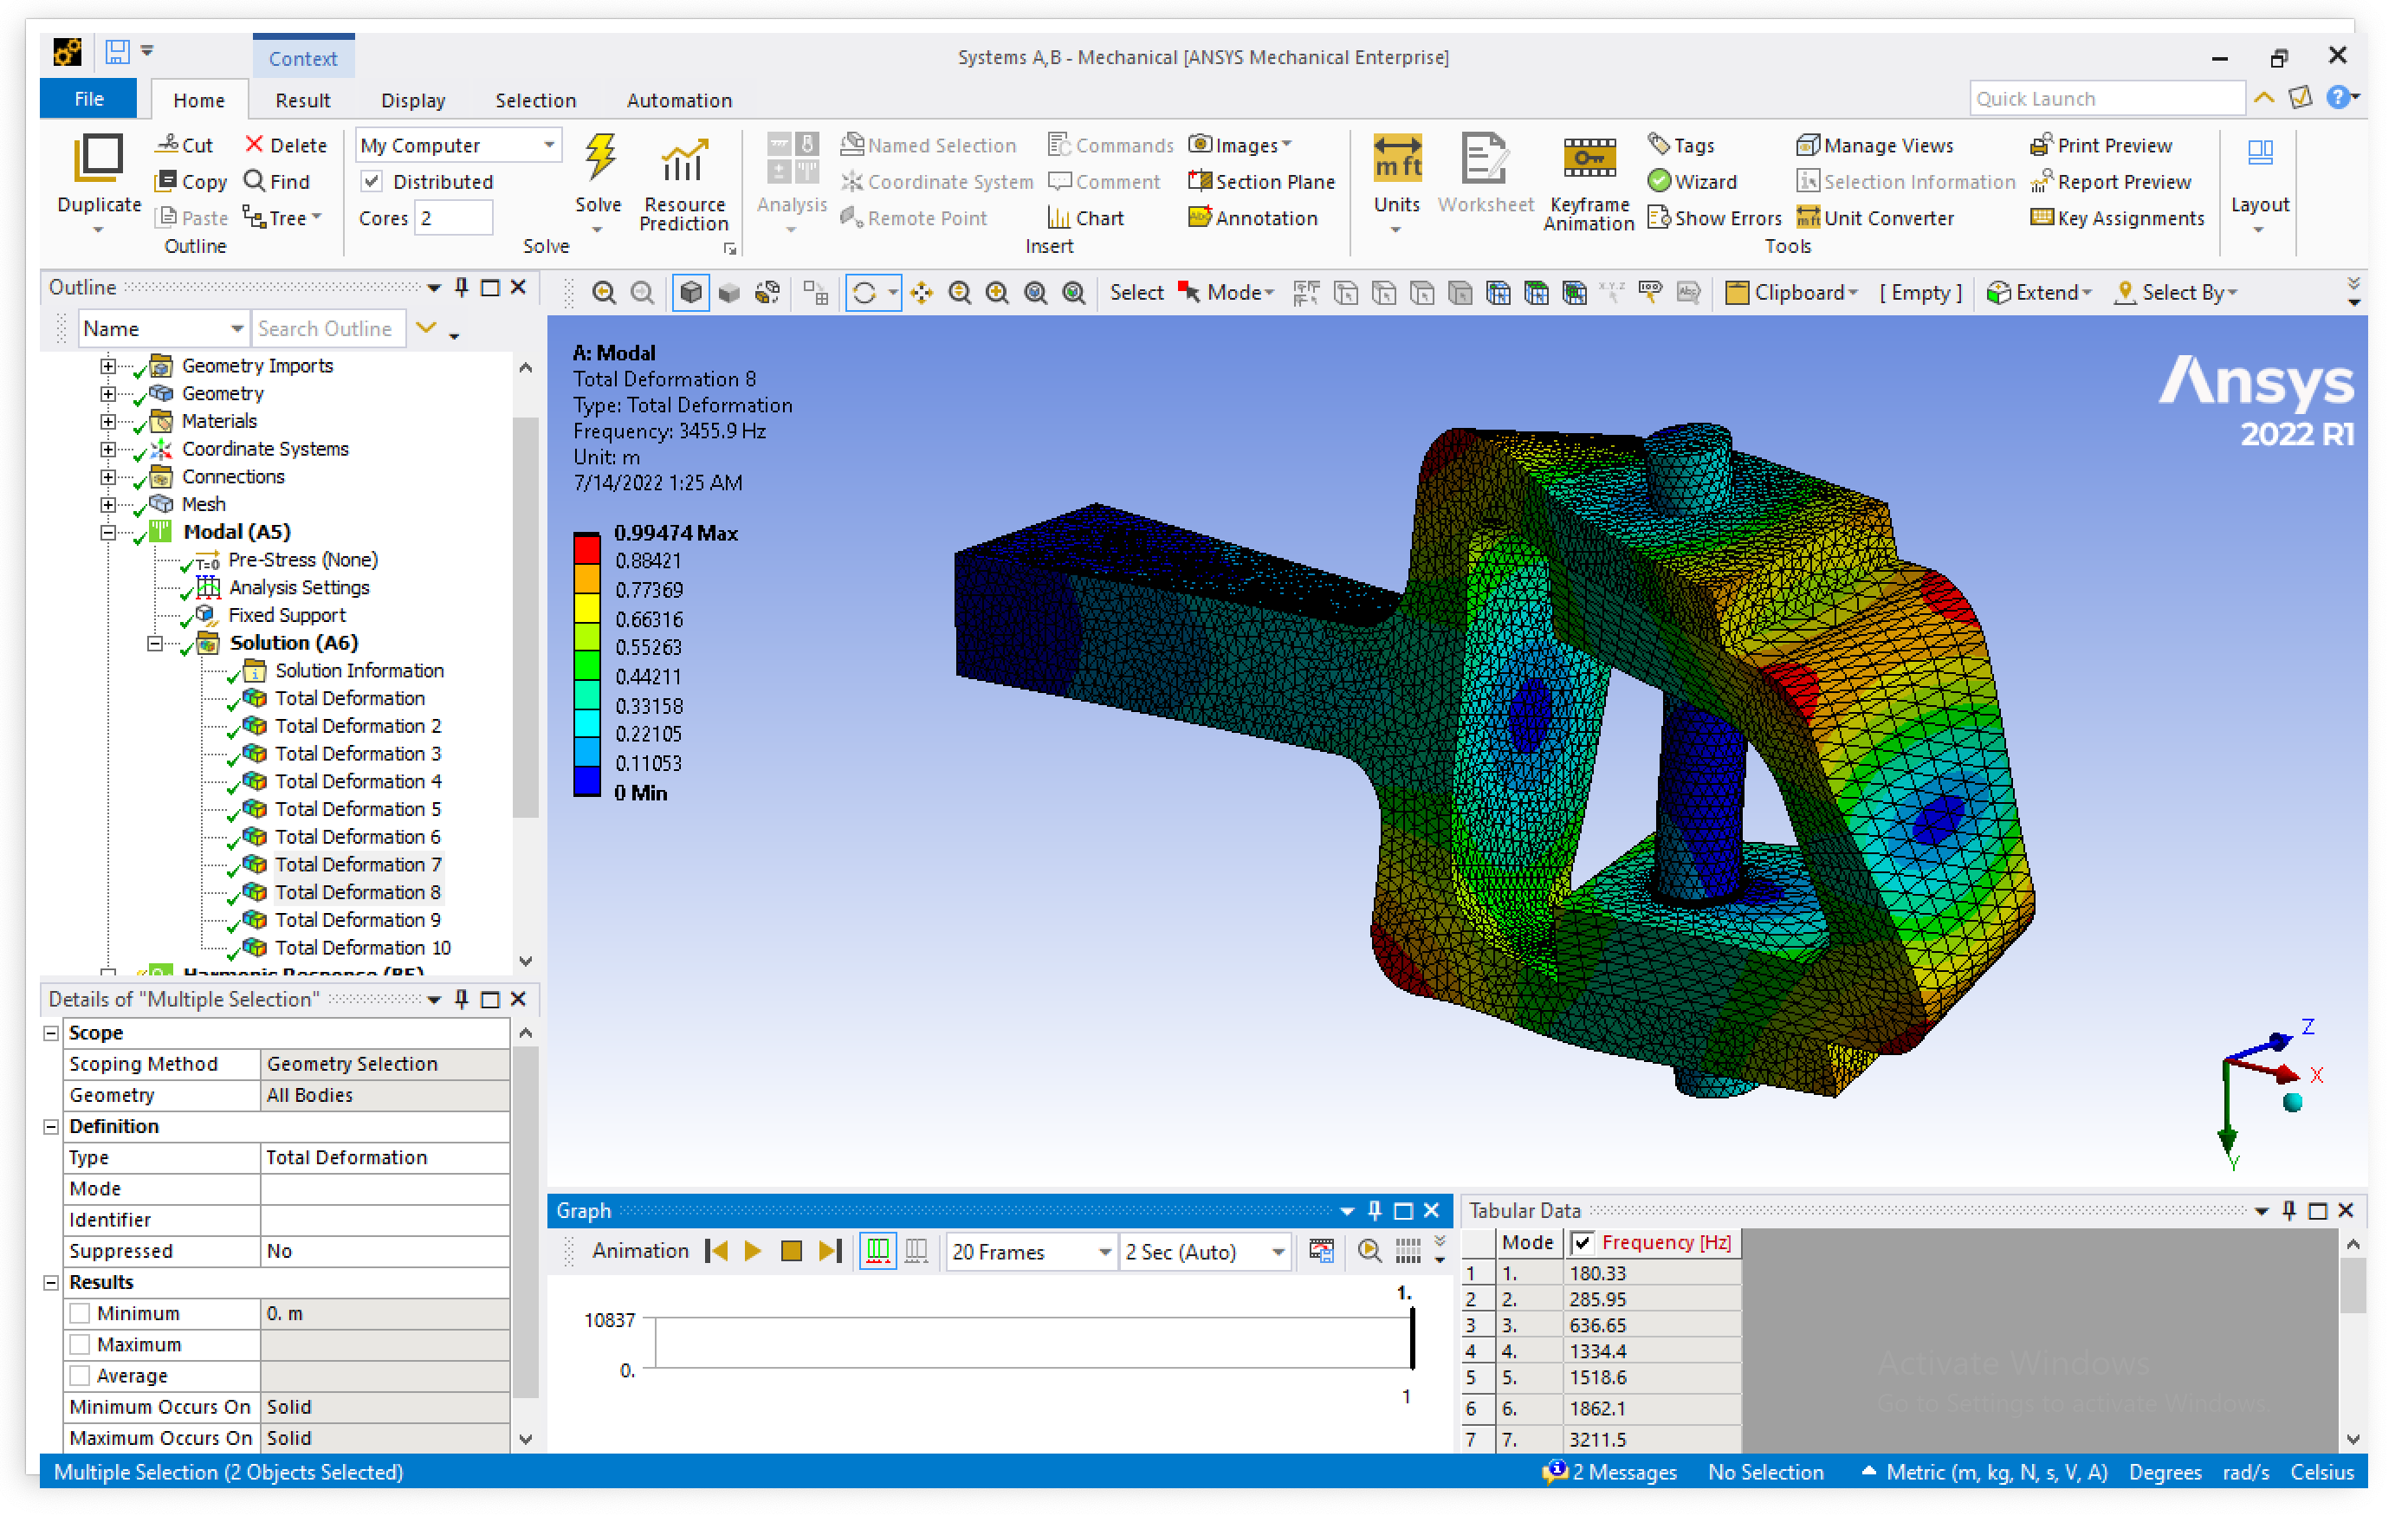
\includegraphics[width=\textwidth]{images/mod8.png}
	\caption{Деформации при восьмой собственной частоте (преимущественно вращение вокруг оси Ox)}
	\label{fig:mod8}
\end{figure}

\begin{figure}[H] 
	\center
	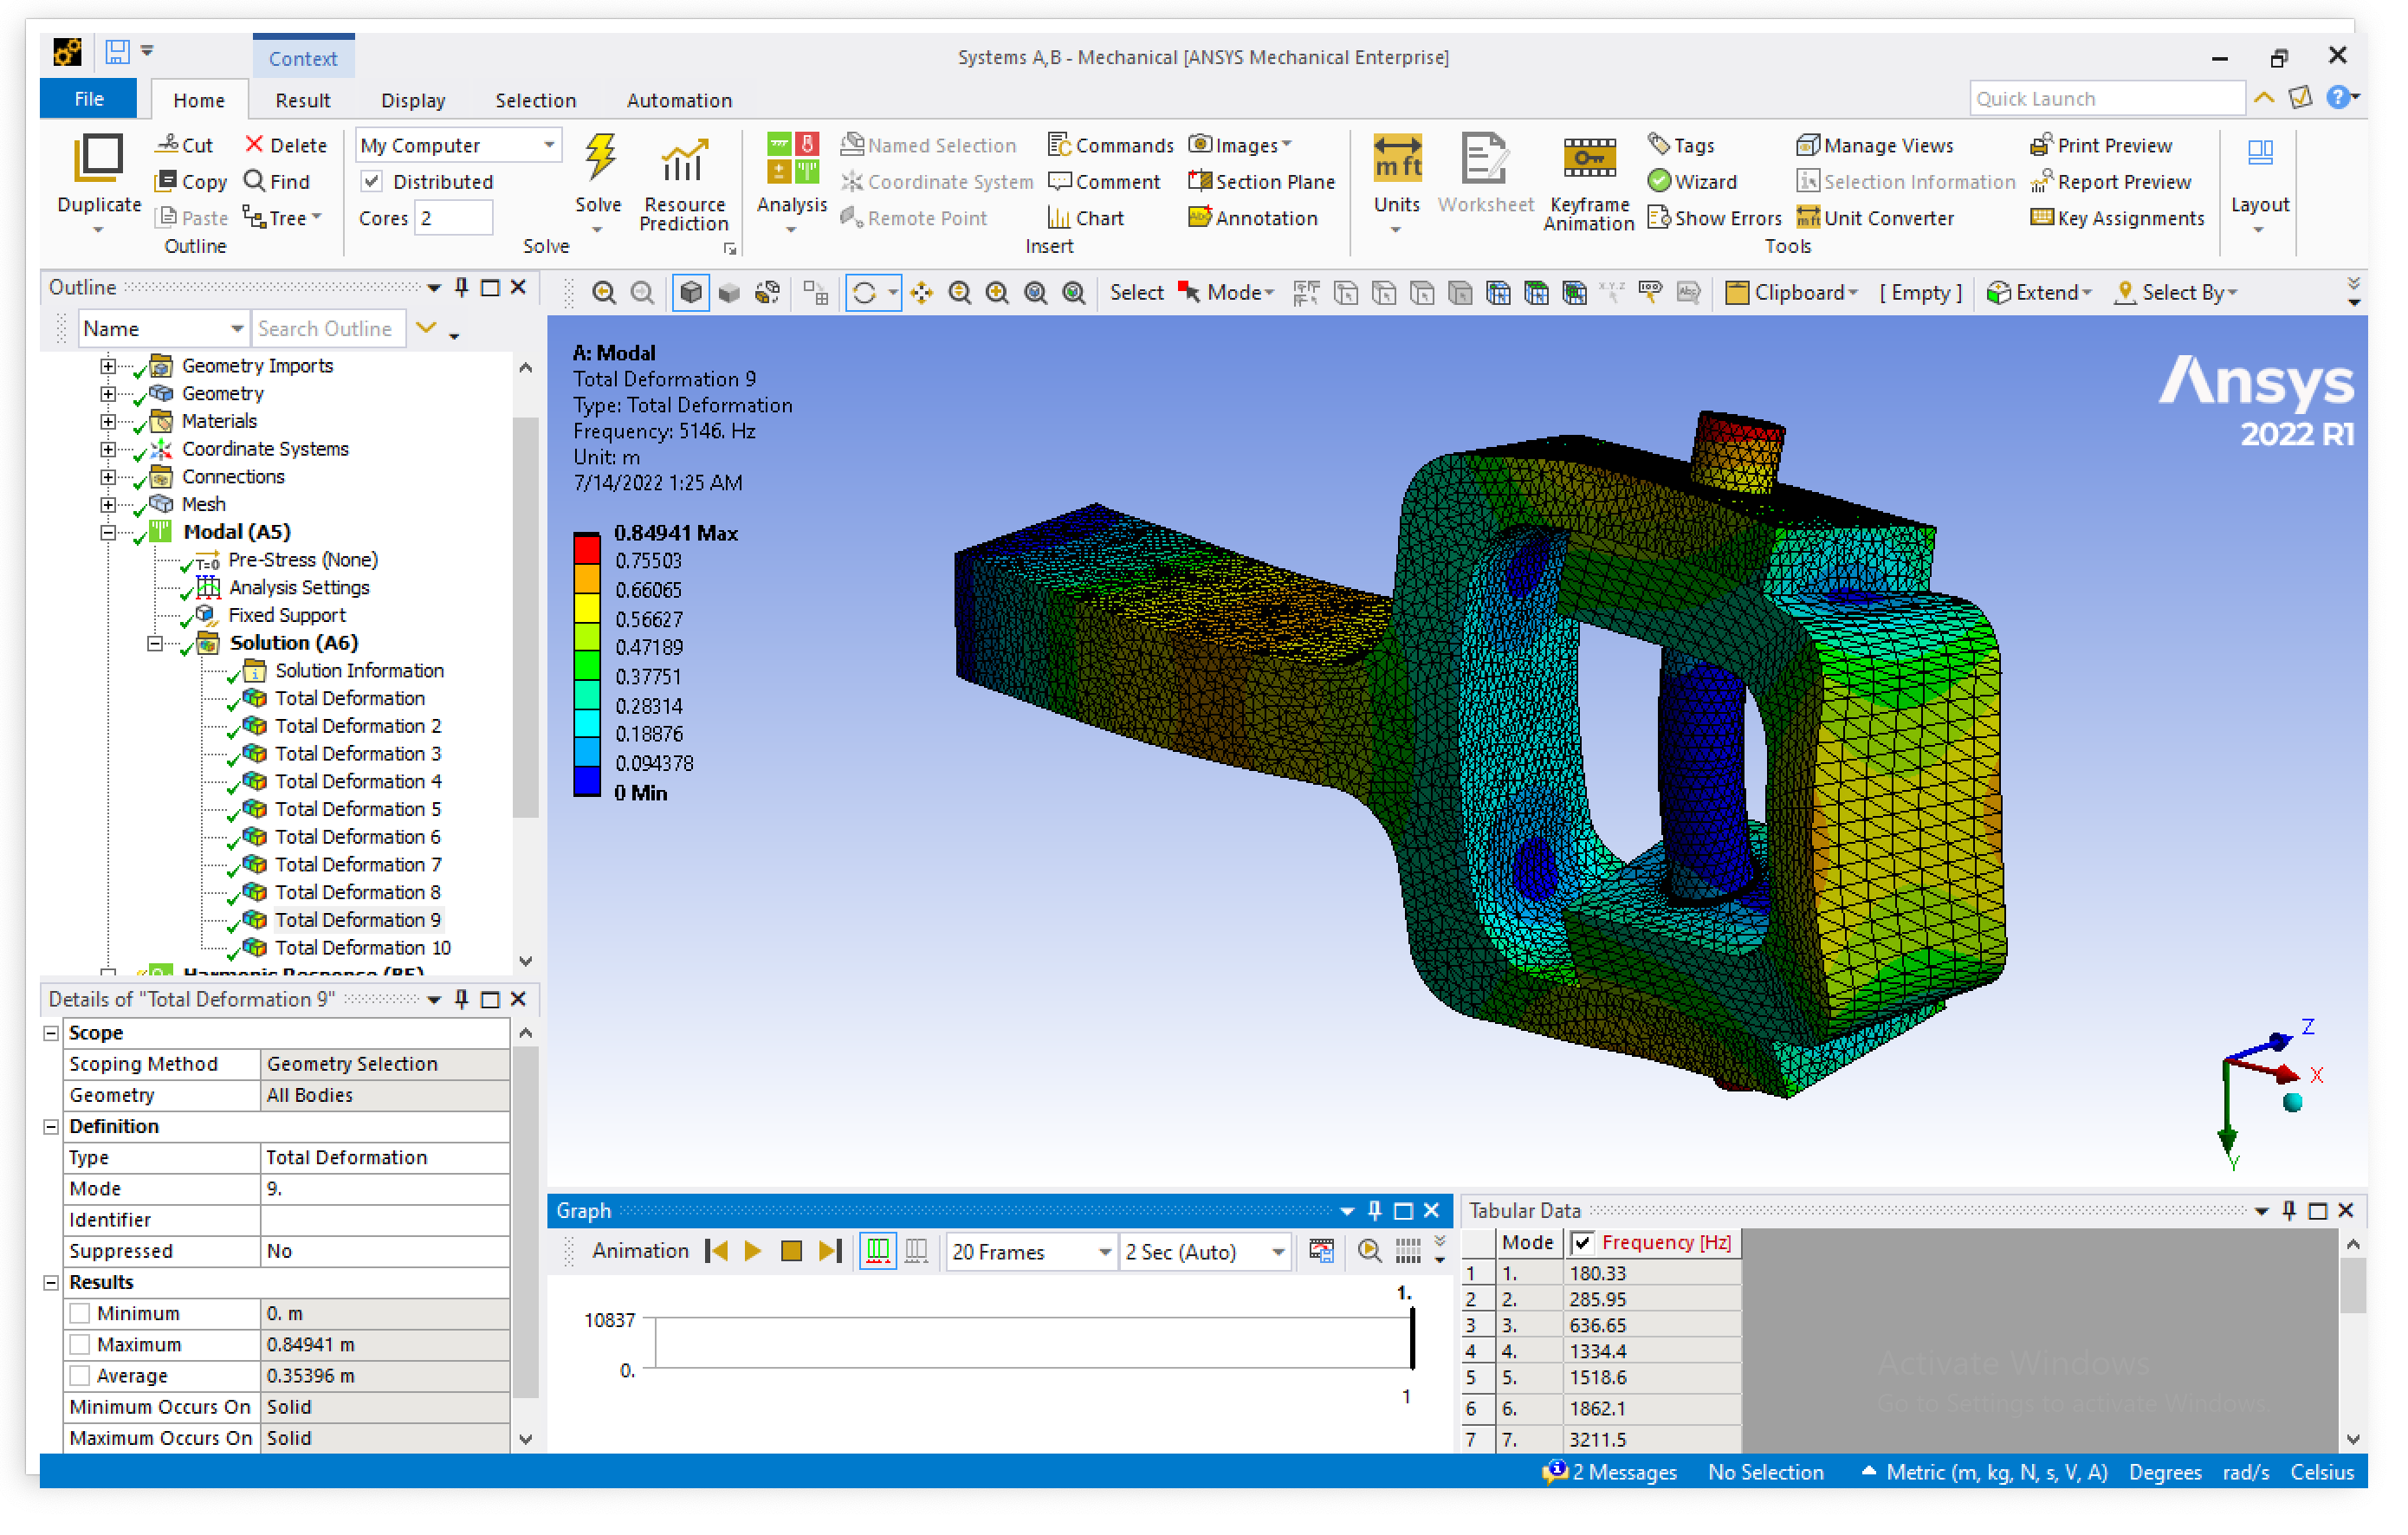
\includegraphics[width=\textwidth]{images/mod9.png}
	\caption{Деформации при девятой собственной частоте (преимущественно перемещение вдоль оси Oz и вращение вокруг оси Oy)}
	\label{fig:mod9}
\end{figure}

\begin{figure}[H] 
	\center
	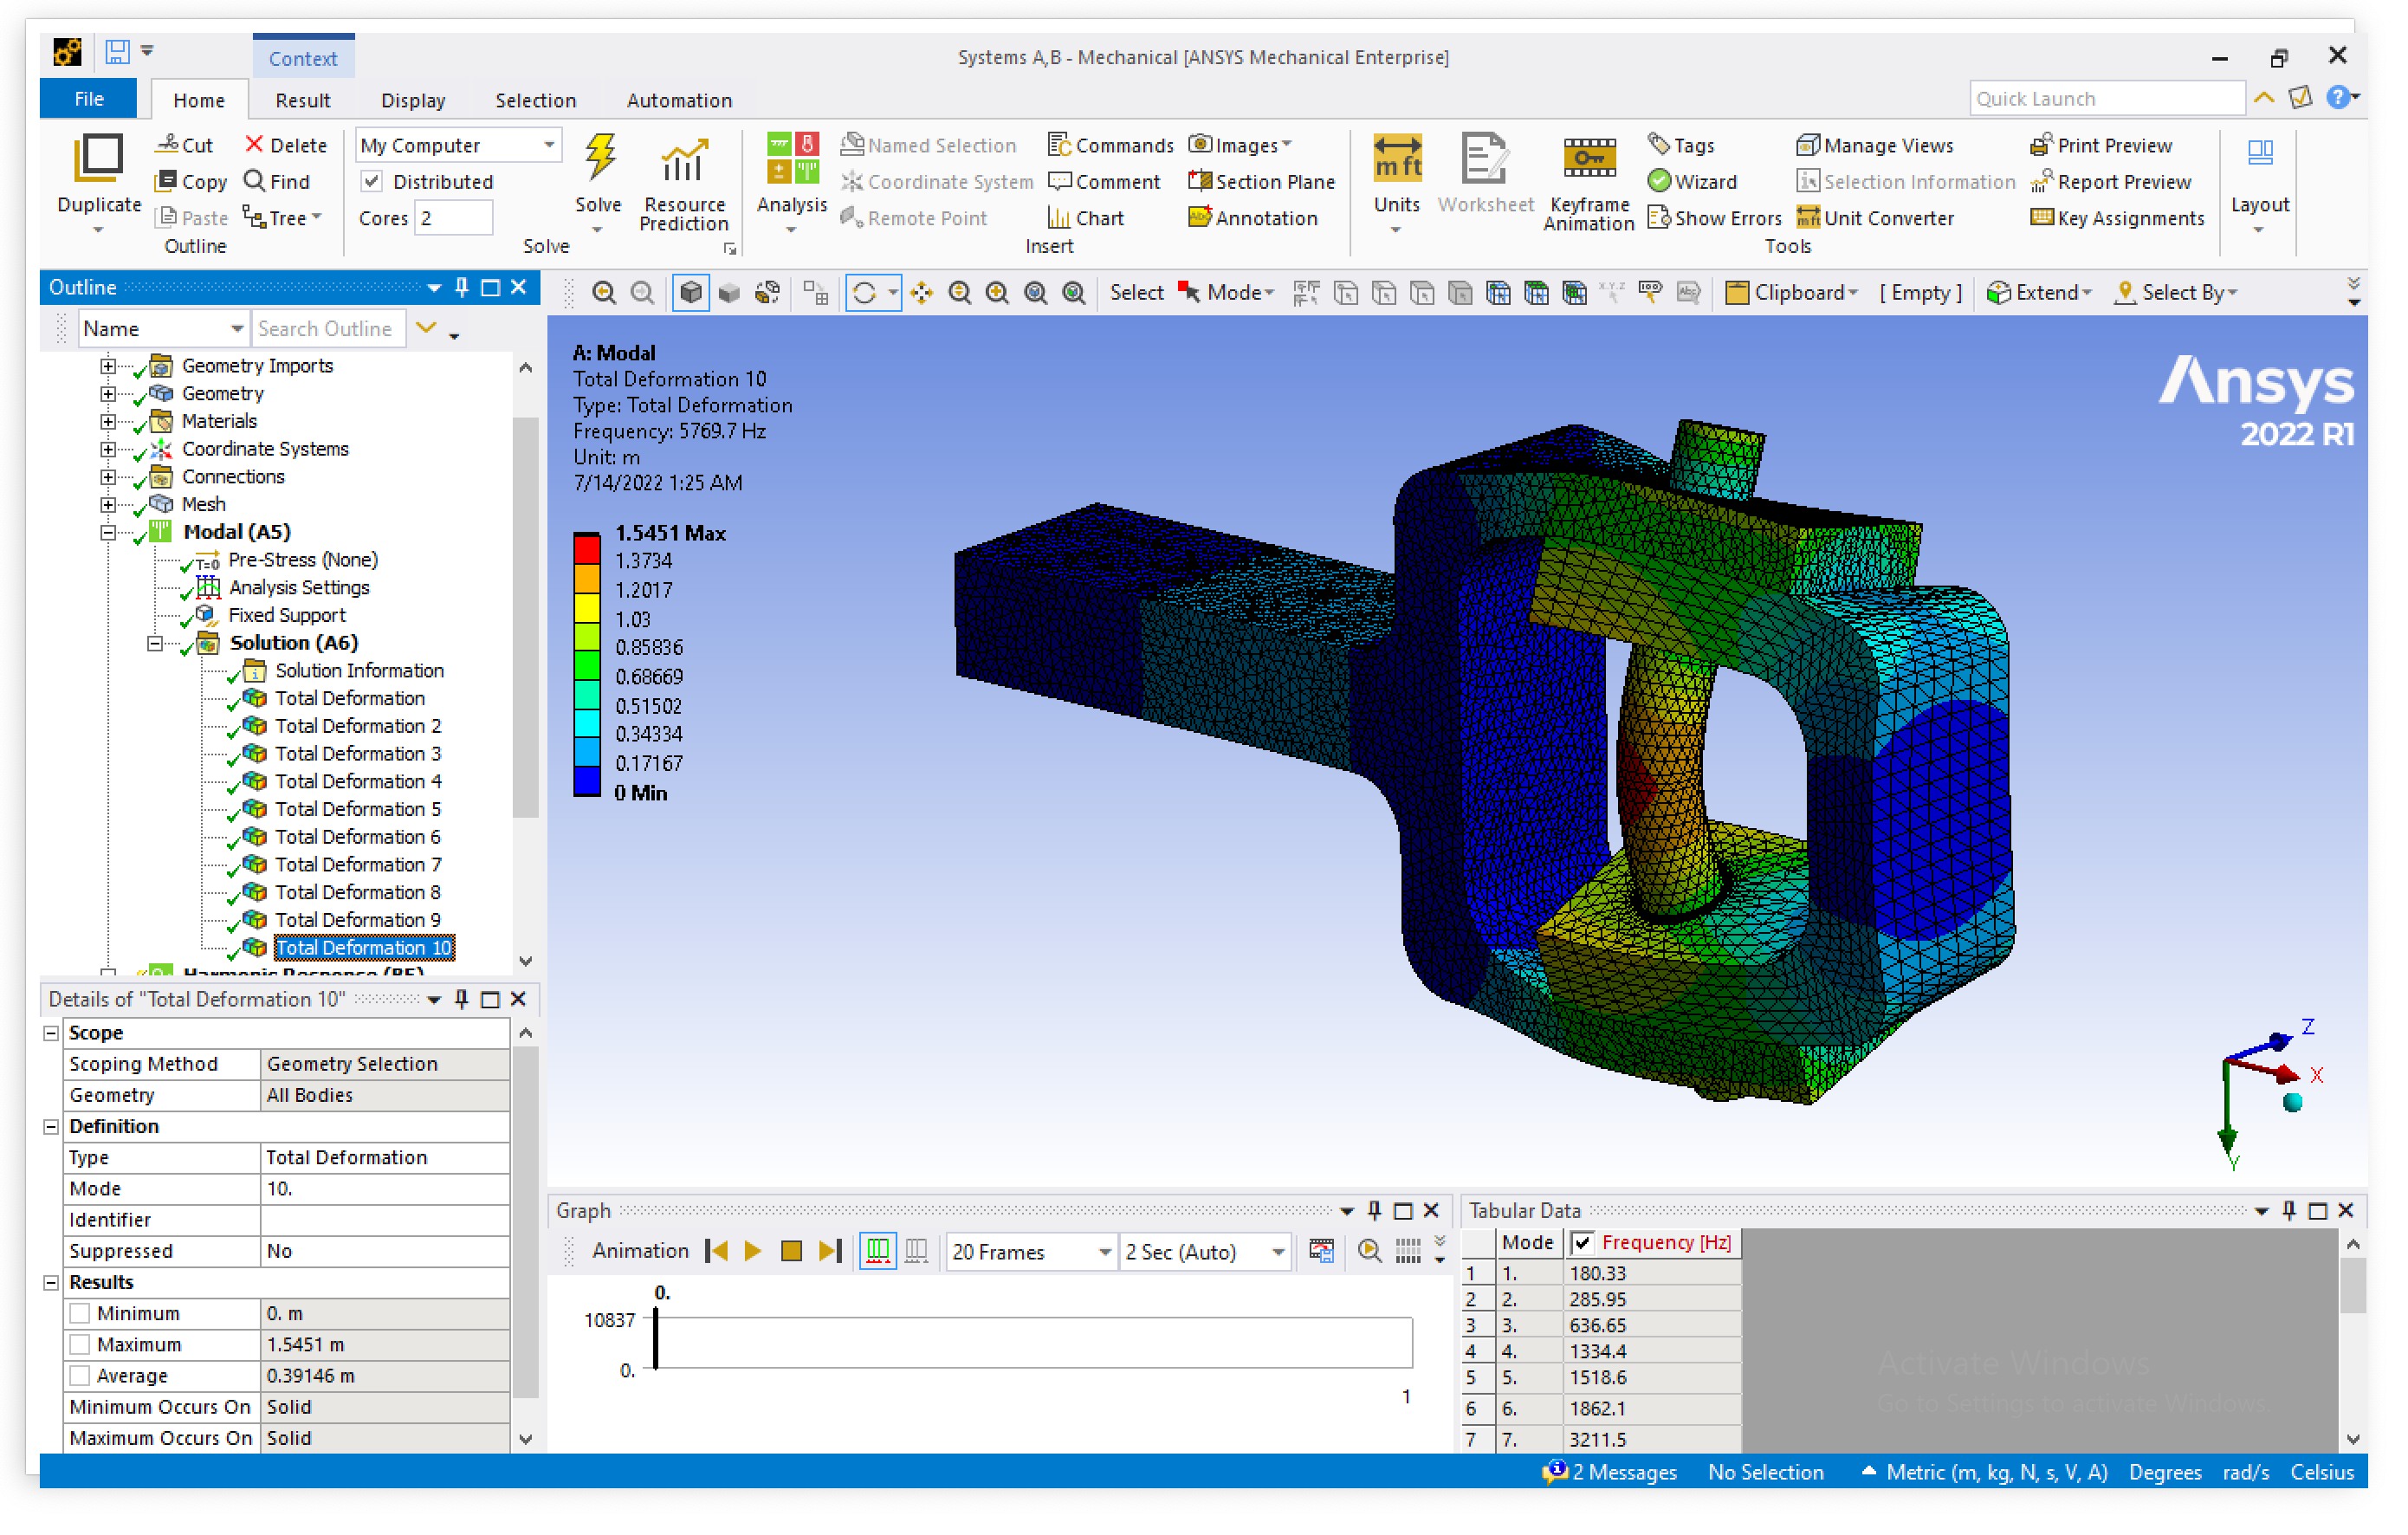
\includegraphics[width=\textwidth]{images/mod10.png}
	\caption{Деформации при десятой собственной частоте (преимущественно перемещение вдоль оси Oz и вращение вокруг оси Oy)}
	\label{fig:mod10}
\end{figure}


Из полученных собственных частот и форм возможно прогнозировать, при каких частотах вибрации следует избегать эксплуатацию рассматриваемого изделия (при эксплуатации на собственных частотах будет резонанс и резко возрастают риски поломки изделия). Значения этих частот для данной геометрии и материала изделия представлены на рис. \ref{fig:frequency_tabular}.

\begin{figure}[H] 
	\center
	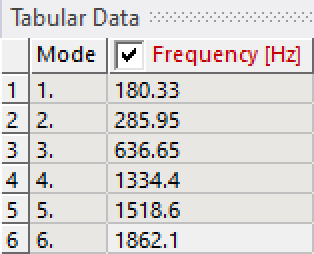
\includegraphics[width=.33\textwidth]{images/frequency_tabular.png}
	\caption{10 первых собственных частот рассматриваемого изделия}
	\label{fig:frequency_tabular}
\end{figure}

Осталось ответить на вопрос: все ли существенные собственные формы извлечены в процессе проведения модального анализа? Для этого построим таблицу отношений эффективных масс к полной массе изделия (рис. \ref{fig:ratio1}).

\begin{figure}[H] 
	\center
	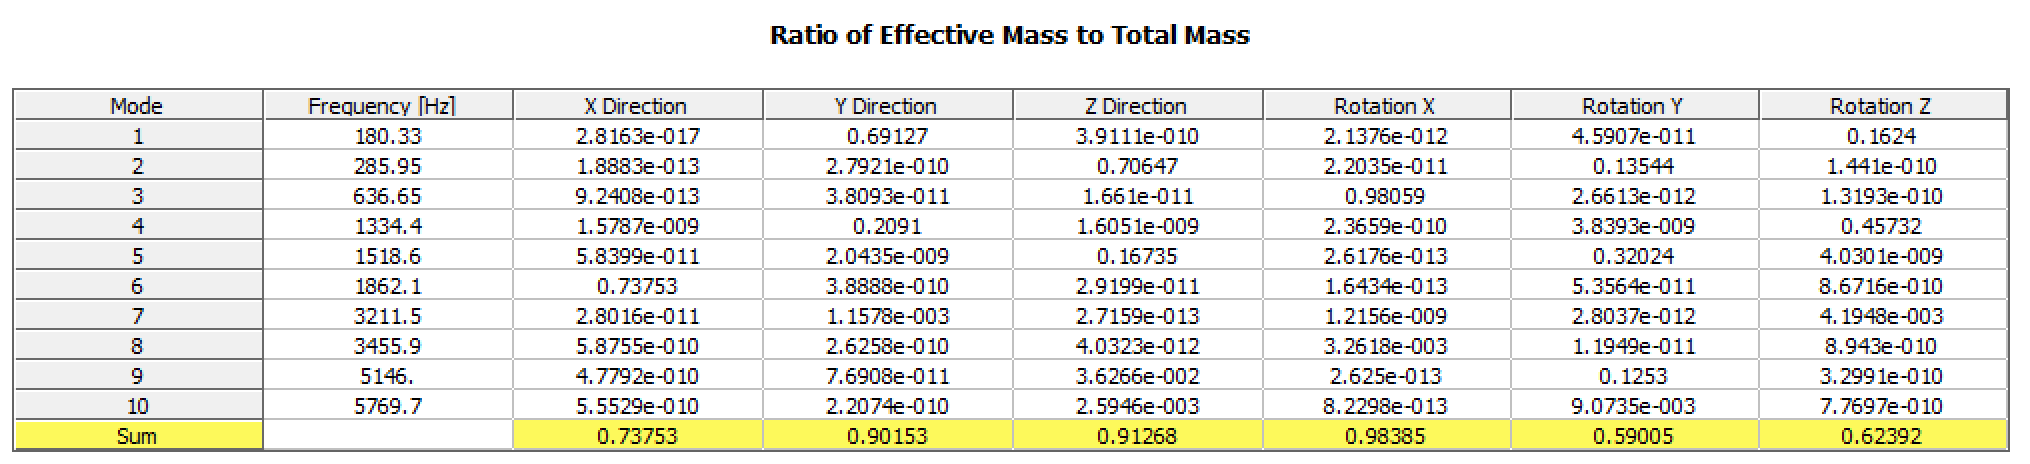
\includegraphics[width=\textwidth]{images/ratio1.png}
	\caption{Отношения эффективных масс к полной массе изделия (10 собственных форм)}
	\label{fig:ratio1}
\end{figure}


Из построенной таблицы видим, что для большинства направлений сумма отношений существенно меньше единицы. Следовательно, требуется извлечь дополнительные собственные формы рассматриваемого изделия.

Таблица отношений эффективных масс к полной массе изделия при извлечении 30 собственных частот представлена на рис. \ref{fig:ratio2}.

\begin{figure}[H] 
	\center
	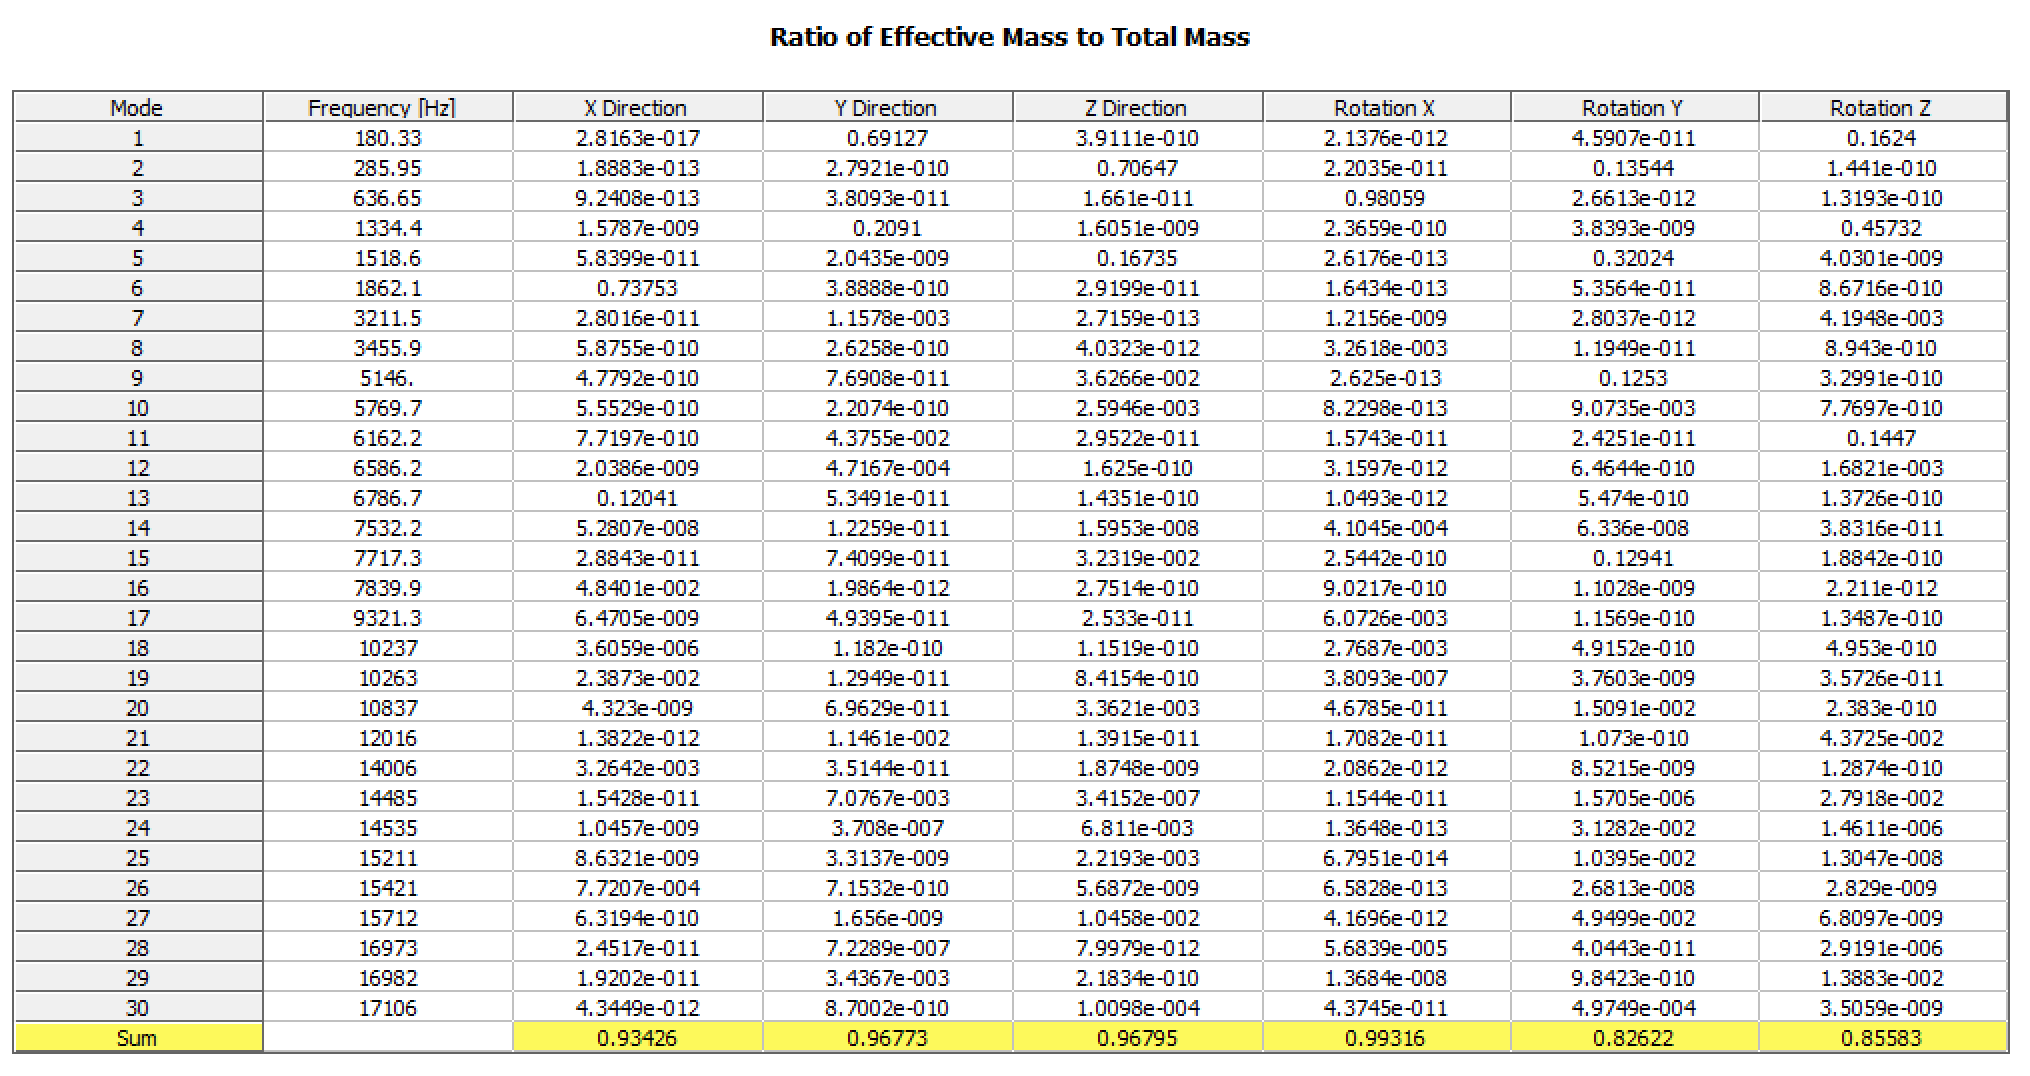
\includegraphics[width=\textwidth]{images/ratio2.png}
	\caption{Отношения эффективных масс к полной массе изделия (30 собственных форм)}
	\label{fig:ratio2}
\end{figure}

Видим, что в первых 30 собственных частотах и формах содержатся наиболее существенные собственные формы рассматриваемого изделия. Но наиболее ёмкие по эффективной массе собственные формы попадают в первые 15 извлечённых собственных форм.
